% Options for packages loaded elsewhere
\PassOptionsToPackage{unicode}{hyperref}
\PassOptionsToPackage{hyphens}{url}
%
\documentclass[
]{article}
\usepackage{lmodern}
\usepackage{amsmath}
\usepackage{ifxetex,ifluatex}
\ifnum 0\ifxetex 1\fi\ifluatex 1\fi=0 % if pdftex
  \usepackage[T1]{fontenc}
  \usepackage[utf8]{inputenc}
  \usepackage{textcomp} % provide euro and other symbols
  \usepackage{amssymb}
\else % if luatex or xetex
  \usepackage{unicode-math}
  \defaultfontfeatures{Scale=MatchLowercase}
  \defaultfontfeatures[\rmfamily]{Ligatures=TeX,Scale=1}
\fi
% Use upquote if available, for straight quotes in verbatim environments
\IfFileExists{upquote.sty}{\usepackage{upquote}}{}
\IfFileExists{microtype.sty}{% use microtype if available
  \usepackage[]{microtype}
  \UseMicrotypeSet[protrusion]{basicmath} % disable protrusion for tt fonts
}{}
\makeatletter
\@ifundefined{KOMAClassName}{% if non-KOMA class
  \IfFileExists{parskip.sty}{%
    \usepackage{parskip}
  }{% else
    \setlength{\parindent}{0pt}
    \setlength{\parskip}{6pt plus 2pt minus 1pt}}
}{% if KOMA class
  \KOMAoptions{parskip=half}}
\makeatother
\usepackage{xcolor}
\IfFileExists{xurl.sty}{\usepackage{xurl}}{} % add URL line breaks if available
\IfFileExists{bookmark.sty}{\usepackage{bookmark}}{\usepackage{hyperref}}
\hypersetup{
  pdftitle={Assignment 6: Entry and Exist},
  pdfauthor={Kohei Kawaguchi},
  hidelinks,
  pdfcreator={LaTeX via pandoc}}
\urlstyle{same} % disable monospaced font for URLs
\usepackage[margin=1in]{geometry}
\usepackage{color}
\usepackage{fancyvrb}
\newcommand{\VerbBar}{|}
\newcommand{\VERB}{\Verb[commandchars=\\\{\}]}
\DefineVerbatimEnvironment{Highlighting}{Verbatim}{commandchars=\\\{\}}
% Add ',fontsize=\small' for more characters per line
\usepackage{framed}
\definecolor{shadecolor}{RGB}{248,248,248}
\newenvironment{Shaded}{\begin{snugshade}}{\end{snugshade}}
\newcommand{\AlertTok}[1]{\textcolor[rgb]{0.94,0.16,0.16}{#1}}
\newcommand{\AnnotationTok}[1]{\textcolor[rgb]{0.56,0.35,0.01}{\textbf{\textit{#1}}}}
\newcommand{\AttributeTok}[1]{\textcolor[rgb]{0.77,0.63,0.00}{#1}}
\newcommand{\BaseNTok}[1]{\textcolor[rgb]{0.00,0.00,0.81}{#1}}
\newcommand{\BuiltInTok}[1]{#1}
\newcommand{\CharTok}[1]{\textcolor[rgb]{0.31,0.60,0.02}{#1}}
\newcommand{\CommentTok}[1]{\textcolor[rgb]{0.56,0.35,0.01}{\textit{#1}}}
\newcommand{\CommentVarTok}[1]{\textcolor[rgb]{0.56,0.35,0.01}{\textbf{\textit{#1}}}}
\newcommand{\ConstantTok}[1]{\textcolor[rgb]{0.00,0.00,0.00}{#1}}
\newcommand{\ControlFlowTok}[1]{\textcolor[rgb]{0.13,0.29,0.53}{\textbf{#1}}}
\newcommand{\DataTypeTok}[1]{\textcolor[rgb]{0.13,0.29,0.53}{#1}}
\newcommand{\DecValTok}[1]{\textcolor[rgb]{0.00,0.00,0.81}{#1}}
\newcommand{\DocumentationTok}[1]{\textcolor[rgb]{0.56,0.35,0.01}{\textbf{\textit{#1}}}}
\newcommand{\ErrorTok}[1]{\textcolor[rgb]{0.64,0.00,0.00}{\textbf{#1}}}
\newcommand{\ExtensionTok}[1]{#1}
\newcommand{\FloatTok}[1]{\textcolor[rgb]{0.00,0.00,0.81}{#1}}
\newcommand{\FunctionTok}[1]{\textcolor[rgb]{0.00,0.00,0.00}{#1}}
\newcommand{\ImportTok}[1]{#1}
\newcommand{\InformationTok}[1]{\textcolor[rgb]{0.56,0.35,0.01}{\textbf{\textit{#1}}}}
\newcommand{\KeywordTok}[1]{\textcolor[rgb]{0.13,0.29,0.53}{\textbf{#1}}}
\newcommand{\NormalTok}[1]{#1}
\newcommand{\OperatorTok}[1]{\textcolor[rgb]{0.81,0.36,0.00}{\textbf{#1}}}
\newcommand{\OtherTok}[1]{\textcolor[rgb]{0.56,0.35,0.01}{#1}}
\newcommand{\PreprocessorTok}[1]{\textcolor[rgb]{0.56,0.35,0.01}{\textit{#1}}}
\newcommand{\RegionMarkerTok}[1]{#1}
\newcommand{\SpecialCharTok}[1]{\textcolor[rgb]{0.00,0.00,0.00}{#1}}
\newcommand{\SpecialStringTok}[1]{\textcolor[rgb]{0.31,0.60,0.02}{#1}}
\newcommand{\StringTok}[1]{\textcolor[rgb]{0.31,0.60,0.02}{#1}}
\newcommand{\VariableTok}[1]{\textcolor[rgb]{0.00,0.00,0.00}{#1}}
\newcommand{\VerbatimStringTok}[1]{\textcolor[rgb]{0.31,0.60,0.02}{#1}}
\newcommand{\WarningTok}[1]{\textcolor[rgb]{0.56,0.35,0.01}{\textbf{\textit{#1}}}}
\usepackage{graphicx}
\makeatletter
\def\maxwidth{\ifdim\Gin@nat@width>\linewidth\linewidth\else\Gin@nat@width\fi}
\def\maxheight{\ifdim\Gin@nat@height>\textheight\textheight\else\Gin@nat@height\fi}
\makeatother
% Scale images if necessary, so that they will not overflow the page
% margins by default, and it is still possible to overwrite the defaults
% using explicit options in \includegraphics[width, height, ...]{}
\setkeys{Gin}{width=\maxwidth,height=\maxheight,keepaspectratio}
% Set default figure placement to htbp
\makeatletter
\def\fps@figure{htbp}
\makeatother
\setlength{\emergencystretch}{3em} % prevent overfull lines
\providecommand{\tightlist}{%
  \setlength{\itemsep}{0pt}\setlength{\parskip}{0pt}}
\setcounter{secnumdepth}{-\maxdimen} % remove section numbering
\ifluatex
  \usepackage{selnolig}  % disable illegal ligatures
\fi

\title{Assignment 6: Entry and Exist}
\author{Kohei Kawaguchi}
\date{}

\begin{document}
\maketitle

\hypertarget{simulate-data}{%
\subsection{Simulate data}\label{simulate-data}}

In this assignment, we consider a Berry-type entry model. Suppose that
there are \(M\) markets indexed by \(m = 1, \cdots, M\). In each market,
there are \(N_m\) potential entrants such that \(N_m \le \overline{N}\).
Let \(x_m\) be the \(K\) dimensional market attributes and \(z_{im}\) be
the \(L\) dimensional potential entrant attributes. The size of Monte
Carlo simulations in the estimation is \(R\).

\begin{enumerate}
\def\labelenumi{\arabic{enumi}.}
\tightlist
\item
  Set the constants as follows:
\end{enumerate}

\begin{Shaded}
\begin{Highlighting}[]
\CommentTok{\# set the seed}
\FunctionTok{set.seed}\NormalTok{(}\DecValTok{1}\NormalTok{)}
\CommentTok{\# number of markets}
\NormalTok{M }\OtherTok{\textless{}{-}} \DecValTok{100}
\CommentTok{\# the upper bound of the number of potential entrants}
\NormalTok{N }\OtherTok{\textless{}{-}} \DecValTok{10}
\CommentTok{\# the dimension of market attributes}
\NormalTok{K }\OtherTok{\textless{}{-}} \DecValTok{2}
\CommentTok{\# the dimension of potential entrant attributes}
\NormalTok{L }\OtherTok{\textless{}{-}} \DecValTok{2}
\CommentTok{\# the number of Monte Carlo simulations}
\NormalTok{R }\OtherTok{\textless{}{-}} \DecValTok{100}
\end{Highlighting}
\end{Shaded}

The payoff of entrant \(i\) in market \(m\) is: \[
\pi_{im}(y_m) = x_m'\beta - \delta \ln \left(\sum_{i = 1}^{N_m} y_{im}\right) + z_{im}'\alpha + \sqrt{1 - \rho^2} \nu_{im} + \rho \epsilon_{m},
\] where \(y_{im} \in \{0, 1\}\) is the indicator for entrant \(i\) in
market \(m\) to enter the market, and \(\nu_{im}\) and \(\epsilon_m\)
are entrant- and market-specific idiosyncratic shocks that are drawn
from an i.i.d. standard normal distribution. In each market, all the
attributes and idiosyncratic shocks are observed by the potential
entrants. \(N_m\), \(x_m\), \(z_{im}\), and \(y_m\) are observed to
econometrician but \(\nu_{im}\) and \(\epsilon_m\) are not.

\begin{enumerate}
\def\labelenumi{\arabic{enumi}.}
\setcounter{enumi}{1}
\tightlist
\item
  Set the parameters as follows:
\end{enumerate}

\begin{Shaded}
\begin{Highlighting}[]
\CommentTok{\# parameters of interest}
\NormalTok{beta }\OtherTok{\textless{}{-}} \FunctionTok{abs}\NormalTok{(}\FunctionTok{rnorm}\NormalTok{(K)); beta}
\end{Highlighting}
\end{Shaded}

\begin{verbatim}
## [1] 0.6264538 0.1836433
\end{verbatim}

\begin{Shaded}
\begin{Highlighting}[]
\NormalTok{alpha }\OtherTok{\textless{}{-}} \FunctionTok{abs}\NormalTok{(}\FunctionTok{rnorm}\NormalTok{(L)); alpha}
\end{Highlighting}
\end{Shaded}

\begin{verbatim}
## [1] 0.8356286 1.5952808
\end{verbatim}

\begin{Shaded}
\begin{Highlighting}[]
\NormalTok{delta }\OtherTok{\textless{}{-}} \DecValTok{1}\NormalTok{; delta}
\end{Highlighting}
\end{Shaded}

\begin{verbatim}
## [1] 1
\end{verbatim}

\begin{Shaded}
\begin{Highlighting}[]
\NormalTok{rho }\OtherTok{\textless{}{-}} \FunctionTok{abs}\NormalTok{(}\FunctionTok{rnorm}\NormalTok{(}\DecValTok{1}\NormalTok{)); rho}
\end{Highlighting}
\end{Shaded}

\begin{verbatim}
## [1] 0.3295078
\end{verbatim}

\begin{Shaded}
\begin{Highlighting}[]
\CommentTok{\# auxiliary parameters}
\NormalTok{x\_mu }\OtherTok{\textless{}{-}} \DecValTok{1}
\NormalTok{x\_sd }\OtherTok{\textless{}{-}} \DecValTok{3}
\NormalTok{z\_mu }\OtherTok{\textless{}{-}} \DecValTok{0}
\NormalTok{z\_sd }\OtherTok{\textless{}{-}} \DecValTok{4}
\end{Highlighting}
\end{Shaded}

\begin{enumerate}
\def\labelenumi{\arabic{enumi}.}
\setcounter{enumi}{2}
\tightlist
\item
  Draw exogenous variables as follows:
\end{enumerate}

\begin{Shaded}
\begin{Highlighting}[]
\CommentTok{\# number of potential entrants}
\NormalTok{E }\OtherTok{\textless{}{-}}\NormalTok{ purrr}\SpecialCharTok{::}\FunctionTok{rdunif}\NormalTok{(M, }\DecValTok{1}\NormalTok{, N); E}
\end{Highlighting}
\end{Shaded}

\begin{verbatim}
##   [1]  3  1  5  5 10  6 10  7  9  5  5  9  9  5  5  2 10  9  1  4  3  6 10 10  6
##  [26]  4  4 10  9  7  6  9  8  9  7  8  6 10  7  3 10  6  8  2  2  6  6  1  3  3
##  [51]  8  6  7  6  8  7  1  4  8  9  9  7  4  7  6  1  5  6  1  9  7  7  3  6  2
##  [76] 10 10  7  3  2 10  1 10 10  8 10  5  7  8  5  6  8  1  3 10  3  1  6  6  4
\end{verbatim}

\begin{Shaded}
\begin{Highlighting}[]
\CommentTok{\# market attributes}
\NormalTok{X }\OtherTok{\textless{}{-}} \FunctionTok{matrix}\NormalTok{(}
  \FunctionTok{rnorm}\NormalTok{(M }\SpecialCharTok{*}\NormalTok{ K, x\_mu, x\_sd),}
  \AttributeTok{nrow =}\NormalTok{ M}
\NormalTok{)}
\FunctionTok{colnames}\NormalTok{(X) }\OtherTok{\textless{}{-}} \FunctionTok{paste}\NormalTok{(}\StringTok{"x"}\NormalTok{, }\DecValTok{1}\SpecialCharTok{:}\NormalTok{K, }\AttributeTok{sep =} \StringTok{"\_"}\NormalTok{)}
\NormalTok{X}
\end{Highlighting}
\end{Shaded}

\begin{verbatim}
##                 x_1          x_2
##   [1,] -0.706006198 -2.693970265
##   [2,]  0.594464155  3.951686710
##   [3,]  4.534260990  1.659774411
##   [4,] -3.570700401 -3.401750087
##   [5,]  2.781838563  2.563068228
##   [6,]  1.998851114  0.523736186
##   [7,]  4.189299512  5.393761936
##   [8,]  0.087448229 -1.298245999
##   [9,]  2.110056430 -0.290635262
##  [10,]  1.801296372 -1.778328492
##  [11,] -0.627560093  0.468688116
##  [12,]  4.623603418  2.206035338
##  [13,]  4.481207847 -1.195244519
##  [14,]  3.100640949  3.491119504
##  [15,]  5.760500364 -2.624248359
##  [16,]  2.675459277 -2.143953238
##  [17,] -2.829776625  5.323473121
##  [18,] -0.719796243 -2.047542396
##  [19,] -2.673837845  2.235924137
##  [20,] -0.420201909 -0.143228153
##  [21,] -0.861100032  2.228205519
##  [22,]  1.126347619  6.066619859
##  [23,] -1.732764946  5.759765300
##  [24,]  1.474086317  0.007276598
##  [25,] -0.963753932 -5.855706606
##  [26,]  6.301861808  8.492984770
##  [27,]  3.150122428  3.001198500
##  [28,]  3.730522688  2.623982008
##  [29,]  2.152556073  0.959801431
##  [30,]  6.046528242  2.530325269
##  [31,] -0.907209362  0.506872505
##  [32,] -0.384934191  2.262083930
##  [33,]  5.296846716 -0.200740232
##  [34,] -0.952089060 -3.110623633
##  [35,]  0.377857769  3.963514802
##  [36,] -0.178423788  5.559235076
##  [37,]  0.040021394  0.073778292
##  [38,]  0.162660091 -2.759869267
##  [39,]  2.482564994  2.926723917
##  [40,]  0.468008553  0.865872589
##  [41,] -0.517872386 -4.199655220
##  [42,]  5.029116476  1.006395579
##  [43,]  0.356261774 -0.890901002
##  [44,]  0.461330410 -0.022905740
##  [45,]  0.699427776 -2.469717088
##  [46,]  3.137998921  6.409425724
##  [47,]  0.779306788  0.006603891
##  [48,]  0.887097486 -3.816540237
##  [49,] -1.044981436  1.591580316
##  [50,]  0.027189183  1.789526939
##  [51,]  1.180481321 -1.957480101
##  [52,] -0.766683459 -7.666762015
##  [53,]  2.594488578 -0.921445108
##  [54,] -3.555182245  2.711522908
##  [55,]  1.919673582  0.820830172
##  [56,] -3.609349471  0.705463768
##  [57,]  0.097071619  2.682462186
##  [58,] -0.584839713 -2.559375916
##  [59,] -0.956284342  4.290331133
##  [60,]  0.829309666  0.983967915
##  [61,] -4.743078277  3.121932002
##  [62,]  4.529749936  4.102323204
##  [63,] -3.994917309  1.670441245
##  [64,] -0.390591204 -1.636122839
##  [65,] -2.347760315  4.488893668
##  [66,] -1.252457004 -5.000494834
##  [67,]  7.261499637 -0.634372220
##  [68,]  1.052186859  0.232987873
##  [69,] -2.858901591  0.501636890
##  [70,] -3.921816603  4.061391726
##  [71,]  2.350561304  1.408665679
##  [72,]  0.944320502  2.221502810
##  [73,]  0.045794876  0.791035561
##  [74,] -1.788086442  0.257006975
##  [75,] -3.462380930  3.086652420
##  [76,] -2.225576890  4.438685072
##  [77,]  4.000086411 -6.209288645
##  [78,] -0.863800084  2.718218666
##  [79,] -3.153280542  2.124173220
##  [80,]  6.607871867 -0.275803165
##  [81,]  2.275301132  3.853038423
##  [82,]  0.284058697 -0.167711545
##  [83,]  4.175449146  0.147008015
##  [84,]  3.659267954  3.572229334
##  [85,] -0.857729145  6.158881897
##  [86,]  7.618307394  1.810164703
##  [87,]  0.234918910 -0.266552029
##  [88,] -3.273483951 -2.567339885
##  [89,]  0.566801194  0.006901063
##  [90,]  1.622615018 -1.819487980
##  [91,]  7.923935197  0.223202251
##  [92,]  1.317407104  2.183137505
##  [93,]  2.370996416 -1.555571276
##  [94,]  0.768541194  8.947500643
##  [95,] -0.002002527  1.468035027
##  [96,]  0.895821915  4.390621802
##  [97,]  3.362918817 -5.867371940
##  [98,]  7.225735026  3.223003472
##  [99,]  4.082177316 -2.948735481
## [100,]  4.623725195  3.759411033
\end{verbatim}

\begin{Shaded}
\begin{Highlighting}[]
\CommentTok{\# entrant attributes}
\NormalTok{Z }\OtherTok{\textless{}{-}}
  \FunctionTok{foreach}\NormalTok{ (}\AttributeTok{m =} \DecValTok{1}\SpecialCharTok{:}\NormalTok{M) }\SpecialCharTok{\%dopar\%}\NormalTok{ \{}
\NormalTok{    Z\_m }\OtherTok{\textless{}{-}} \FunctionTok{matrix}\NormalTok{(}
      \FunctionTok{rnorm}\NormalTok{(E[m] }\SpecialCharTok{*}\NormalTok{ L, z\_mu, z\_sd),}
      \AttributeTok{nrow =}\NormalTok{ E[m]}
\NormalTok{    )}
    \FunctionTok{colnames}\NormalTok{(Z\_m) }\OtherTok{\textless{}{-}} \FunctionTok{paste}\NormalTok{(}\StringTok{"z"}\NormalTok{, }\DecValTok{1}\SpecialCharTok{:}\NormalTok{L, }\AttributeTok{sep =} \StringTok{"\_"}\NormalTok{)}
    \FunctionTok{return}\NormalTok{(Z\_m)}
\NormalTok{  \}}
\NormalTok{Z[[}\DecValTok{1}\NormalTok{]]}
\end{Highlighting}
\end{Shaded}

\begin{verbatim}
##            z_1        z_2
## [1,] -2.081654 -4.9299861
## [2,] -2.100983 -7.4086994
## [3,] -1.625720 -0.9564999
\end{verbatim}

\begin{Shaded}
\begin{Highlighting}[]
\CommentTok{\# unobserved market attributes}
\NormalTok{EP }\OtherTok{\textless{}{-}} \FunctionTok{matrix}\NormalTok{(}
  \FunctionTok{rnorm}\NormalTok{(M),}
  \AttributeTok{nrow =}\NormalTok{ M}
\NormalTok{)}
\NormalTok{EP}
\end{Highlighting}
\end{Shaded}

\begin{verbatim}
##                [,1]
##   [1,]  0.398130155
##   [2,] -0.407528579
##   [3,]  1.324258630
##   [4,] -0.701231669
##   [5,] -0.580614304
##   [6,] -1.001072181
##   [7,] -0.668178607
##   [8,]  0.945184953
##   [9,]  0.433702150
##  [10,]  1.005159218
##  [11,] -0.390118664
##  [12,]  0.376370292
##  [13,]  0.244164924
##  [14,] -1.426257342
##  [15,]  1.778429287
##  [16,]  0.134447661
##  [17,]  0.765598999
##  [18,]  0.955136677
##  [19,] -0.050565701
##  [20,] -0.305815420
##  [21,]  0.893673702
##  [22,] -1.047298149
##  [23,]  1.971337386
##  [24,] -0.383632106
##  [25,]  1.654145302
##  [26,]  1.512212694
##  [27,]  0.082965734
##  [28,]  0.567220915
##  [29,] -1.024548480
##  [30,]  0.323006503
##  [31,]  1.043612458
##  [32,]  0.099078487
##  [33,] -0.454136909
##  [34,] -0.655781852
##  [35,] -0.035922423
##  [36,]  1.069161461
##  [37,] -0.483974930
##  [38,] -0.121010111
##  [39,] -1.294140004
##  [40,]  0.494312836
##  [41,]  1.307901520
##  [42,]  1.497041009
##  [43,]  0.814702731
##  [44,] -1.869788790
##  [45,]  0.482029504
##  [46,]  0.456135603
##  [47,] -0.353400286
##  [48,]  0.170489471
##  [49,] -0.864035954
##  [50,]  0.679230774
##  [51,] -0.327101015
##  [52,] -1.569082185
##  [53,] -0.367450756
##  [54,]  1.364434929
##  [55,] -0.334281365
##  [56,]  0.732750042
##  [57,]  0.946585640
##  [58,]  0.004398704
##  [59,] -0.352322306
##  [60,] -0.529695509
##  [61,]  0.739589226
##  [62,] -1.063457415
##  [63,]  0.246210844
##  [64,] -0.289499367
##  [65,] -2.264889356
##  [66,] -1.408850456
##  [67,]  0.916019329
##  [68,] -0.191278951
##  [69,]  0.803283216
##  [70,]  1.887474463
##  [71,]  1.473881181
##  [72,]  0.677268492
##  [73,]  0.379962687
##  [74,] -0.192798426
##  [75,]  1.577891795
##  [76,]  0.596234109
##  [77,] -1.173576941
##  [78,] -0.155642535
##  [79,] -1.918909820
##  [80,] -0.195258846
##  [81,] -2.592327670
##  [82,]  1.314002167
##  [83,] -0.635543001
##  [84,] -0.429978839
##  [85,] -0.169318332
##  [86,]  0.612218174
##  [87,]  0.678340177
##  [88,]  0.567951972
##  [89,] -0.572542604
##  [90,] -1.363291256
##  [91,] -0.388722244
##  [92,]  0.277914132
##  [93,] -0.823081122
##  [94,] -0.068840934
##  [95,] -1.167662326
##  [96,] -0.008309014
##  [97,]  0.128855402
##  [98,] -0.145875628
##  [99,] -0.163910957
## [100,]  1.763552003
\end{verbatim}

\begin{Shaded}
\begin{Highlighting}[]
\CommentTok{\# unobserved entrant attributes}
\NormalTok{NU }\OtherTok{\textless{}{-}}
  \FunctionTok{foreach}\NormalTok{ (}\AttributeTok{m =} \DecValTok{1}\SpecialCharTok{:}\NormalTok{M) }\SpecialCharTok{\%dopar\%}\NormalTok{ \{}
\NormalTok{    NU\_m }\OtherTok{\textless{}{-}} \FunctionTok{matrix}\NormalTok{(}
      \FunctionTok{rnorm}\NormalTok{(E[m]),}
      \AttributeTok{nrow =}\NormalTok{ E[m]}
\NormalTok{    )}
    \FunctionTok{return}\NormalTok{(NU\_m)}
\NormalTok{  \}}
\NormalTok{NU[[}\DecValTok{1}\NormalTok{]]}
\end{Highlighting}
\end{Shaded}

\begin{verbatim}
##             [,1]
## [1,]  1.20846499
## [2,]  0.06999019
## [3,] -2.05651414
\end{verbatim}

\begin{enumerate}
\def\labelenumi{\arabic{enumi}.}
\setcounter{enumi}{3}
\tightlist
\item
  Write a function
  \texttt{compute\_payoff(y\_m,\ X\_m,\ Z\_m,\ EP\_m,\ NU\_m,\ beta,\ alpha,\ delta,\ rho)}
  that returns the vector of payoffs of the potential entrants when the
  vector of entry decisions is \texttt{y\_m}.
\end{enumerate}

\begin{Shaded}
\begin{Highlighting}[]
\CommentTok{\# compute payoff}
\NormalTok{compute\_payoff }\OtherTok{\textless{}{-}}
  \ControlFlowTok{function}\NormalTok{(y\_m, X\_m, Z\_m, EP\_m, NU\_m, beta, alpha, delta, rho) \{}
\NormalTok{    N\_m }\OtherTok{\textless{}{-}} \FunctionTok{length}\NormalTok{(y\_m)}
    \ControlFlowTok{if}\NormalTok{ (}\FunctionTok{sum}\NormalTok{(y\_m) }\SpecialCharTok{==} \DecValTok{0}\NormalTok{) \{}
\NormalTok{      payoff\_m }\OtherTok{\textless{}{-}} \DecValTok{0} \SpecialCharTok{*}\NormalTok{ y\_m}
\NormalTok{    \} }\ControlFlowTok{else}\NormalTok{ \{}
\NormalTok{      payoff\_m }\OtherTok{\textless{}{-}} \FunctionTok{matrix}\NormalTok{(}\FunctionTok{rep}\NormalTok{(}\DecValTok{1}\NormalTok{, N\_m)) }\SpecialCharTok{\%*\%}\NormalTok{ (X\_m }\SpecialCharTok{\%*\%}\NormalTok{ beta }\SpecialCharTok{{-}}\NormalTok{ delta }\SpecialCharTok{*} \FunctionTok{log}\NormalTok{(}\FunctionTok{sum}\NormalTok{(y\_m)) }\SpecialCharTok{+}\NormalTok{ rho }\SpecialCharTok{*}\NormalTok{ EP\_m) }\SpecialCharTok{+}\NormalTok{ Z\_m }\SpecialCharTok{\%*\%}\NormalTok{ alpha }\SpecialCharTok{+} \FunctionTok{sqrt}\NormalTok{(}\DecValTok{1} \SpecialCharTok{{-}}\NormalTok{ rho}\SpecialCharTok{\^{}}\DecValTok{2}\NormalTok{) }\SpecialCharTok{*}\NormalTok{ NU\_m }
\NormalTok{      payoff\_m }\OtherTok{\textless{}{-}}\NormalTok{ payoff\_m }\SpecialCharTok{*}\NormalTok{ y\_m}
\NormalTok{    \}}
    \FunctionTok{return}\NormalTok{(payoff\_m)}
\NormalTok{  \}}
\NormalTok{m }\OtherTok{\textless{}{-}} \DecValTok{1}
\NormalTok{N\_m }\OtherTok{\textless{}{-}} \FunctionTok{dim}\NormalTok{(Z[[m]])[}\DecValTok{1}\NormalTok{]}
\NormalTok{y\_m }\OtherTok{\textless{}{-}} \FunctionTok{as.matrix}\NormalTok{(}\FunctionTok{rep}\NormalTok{(}\DecValTok{1}\NormalTok{, N\_m))}
\NormalTok{y\_m[}\FunctionTok{length}\NormalTok{(y\_m)] }\OtherTok{\textless{}{-}} \DecValTok{0}
\NormalTok{X\_m }\OtherTok{\textless{}{-}}\NormalTok{ X[m, , drop }\OtherTok{=} \ConstantTok{FALSE}\NormalTok{]}
\NormalTok{Z\_m }\OtherTok{\textless{}{-}}\NormalTok{ Z[[m]]}
\NormalTok{EP\_m }\OtherTok{\textless{}{-}}\NormalTok{ EP[m, , drop }\OtherTok{=} \ConstantTok{FALSE}\NormalTok{]}
\NormalTok{NU\_m }\OtherTok{\textless{}{-}}\NormalTok{ NU[[m]]}
\FunctionTok{compute\_payoff}\NormalTok{(y\_m, X\_m, Z\_m, EP\_m, NU\_m, beta, alpha, delta, rho)}
\end{Highlighting}
\end{Shaded}

\begin{verbatim}
##            [,1]
## [1,]  -9.962196
## [2,] -15.007486
## [3,]   0.000000
\end{verbatim}

\begin{enumerate}
\def\labelenumi{\arabic{enumi}.}
\setcounter{enumi}{4}
\tightlist
\item
  Assume that the order of entry is predetermined. Assume that the
  potential entrants sequentially decide entry according to the order of
  the payoff excluding the competitive effects, i.e.: \[
  x_m'\beta + z_{im}'\alpha + \sqrt{1 - \rho^2} \nu_{im} + \rho \epsilon_{m}.
  \] Write a function
  \texttt{compute\_sequential\_entry(X\_m,\ Z\_m,\ EP\_m,\ NU\_m,\ beta,\ alpha,\ delta,\ rho)}
  that returns the equilibrium vector of entry at a market.
\end{enumerate}

\begin{Shaded}
\begin{Highlighting}[]
\CommentTok{\# compute sequential entry}
\NormalTok{compute\_sequential\_entry }\OtherTok{\textless{}{-}}
  \ControlFlowTok{function}\NormalTok{(X\_m, Z\_m, EP\_m, NU\_m, beta, alpha, delta, rho) \{}
\NormalTok{    N\_m }\OtherTok{\textless{}{-}} \FunctionTok{dim}\NormalTok{(Z\_m)[}\DecValTok{1}\NormalTok{]}
\NormalTok{    y\_m }\OtherTok{\textless{}{-}} \FunctionTok{rep}\NormalTok{(}\DecValTok{0}\NormalTok{, N\_m)}
\NormalTok{    N\_m }\OtherTok{\textless{}{-}} \FunctionTok{dim}\NormalTok{(Z\_m)[}\DecValTok{1}\NormalTok{]}
    \CommentTok{\# compute the baseline payoff}
\NormalTok{    payoff\_baseline }\OtherTok{\textless{}{-}} \FunctionTok{matrix}\NormalTok{(}\FunctionTok{rep}\NormalTok{(}\DecValTok{1}\NormalTok{, N\_m)) }\SpecialCharTok{\%*\%}\NormalTok{ (X\_m }\SpecialCharTok{\%*\%}\NormalTok{ beta }\SpecialCharTok{+}\NormalTok{ rho }\SpecialCharTok{*}\NormalTok{ EP\_m) }\SpecialCharTok{+}\NormalTok{ Z\_m }\SpecialCharTok{\%*\%}\NormalTok{ alpha }\SpecialCharTok{+} \FunctionTok{sqrt}\NormalTok{(}\DecValTok{1} \SpecialCharTok{{-}}\NormalTok{ rho}\SpecialCharTok{\^{}}\DecValTok{2}\NormalTok{) }\SpecialCharTok{*}\NormalTok{ NU\_m }
    \CommentTok{\# baseline payoff ranking}
\NormalTok{    ranking }\OtherTok{\textless{}{-}} \FunctionTok{rank}\NormalTok{(}\SpecialCharTok{{-}}\NormalTok{payoff\_baseline)}
    \CommentTok{\# initial y\_m}
\NormalTok{    y\_m }\OtherTok{\textless{}{-}} \FunctionTok{rep}\NormalTok{(}\DecValTok{0}\NormalTok{, N\_m)}
    \ControlFlowTok{for}\NormalTok{ (index }\ControlFlowTok{in} \DecValTok{1}\SpecialCharTok{:}\NormalTok{N\_m) \{}
\NormalTok{      i }\OtherTok{\textless{}{-}} \FunctionTok{which}\NormalTok{(ranking }\SpecialCharTok{==}\NormalTok{ index)}
\NormalTok{      y\_m0 }\OtherTok{\textless{}{-}}\NormalTok{ y\_m}
\NormalTok{      y\_m0[i] }\OtherTok{\textless{}{-}} \DecValTok{1}
\NormalTok{      payoff }\OtherTok{\textless{}{-}} \FunctionTok{compute\_payoff}\NormalTok{(y\_m0, X\_m, Z\_m, EP\_m, NU\_m, beta, alpha, delta, rho)}
\NormalTok{      payoff\_i }\OtherTok{\textless{}{-}}\NormalTok{ payoff[i]}
\NormalTok{      y\_m[i] }\OtherTok{\textless{}{-}} \FunctionTok{as.integer}\NormalTok{(payoff\_i }\SpecialCharTok{\textgreater{}=} \DecValTok{0}\NormalTok{)}
\NormalTok{    \}}
\NormalTok{    y\_m }\OtherTok{\textless{}{-}} \FunctionTok{as.matrix}\NormalTok{(y\_m)}
    \FunctionTok{return}\NormalTok{(y\_m)}
\NormalTok{  \}}
\FunctionTok{compute\_sequential\_entry}\NormalTok{(X\_m, Z\_m, EP\_m, NU\_m, beta, alpha, delta, rho)}
\end{Highlighting}
\end{Shaded}

\begin{verbatim}
##      [,1]
## [1,]    0
## [2,]    0
## [3,]    0
\end{verbatim}

\begin{enumerate}
\def\labelenumi{\arabic{enumi}.}
\setcounter{enumi}{5}
\tightlist
\item
  Next, assume \(\rho = 0\). Assume that potential entrants
  simultaneously decide entry. Write a function
  \texttt{compute\_simultaneous\_entry(X\_m,\ Z\_m,\ EP\_m,\ NU\_m,\ beta,\ alpha,\ delta)}
  that returns the equilibrium vector of entry at a market.
\end{enumerate}

\begin{Shaded}
\begin{Highlighting}[]
\CommentTok{\# compute simultaneous entry}
\NormalTok{compute\_simultaneous\_entry }\OtherTok{\textless{}{-}}
  \ControlFlowTok{function}\NormalTok{(X\_m, Z\_m, EP\_m, NU\_m, beta, alpha, delta) \{}
\NormalTok{    N\_m }\OtherTok{\textless{}{-}} \FunctionTok{dim}\NormalTok{(Z\_m)[}\DecValTok{1}\NormalTok{]}
\NormalTok{    y\_m }\OtherTok{\textless{}{-}} \FunctionTok{rep}\NormalTok{(}\DecValTok{1}\NormalTok{, N\_m)}
\NormalTok{    y\_m\_old }\OtherTok{\textless{}{-}} \FunctionTok{rep}\NormalTok{(}\DecValTok{0}\NormalTok{, N\_m)}
    \ControlFlowTok{while}\NormalTok{ (}\SpecialCharTok{!}\FunctionTok{identical}\NormalTok{(y\_m, y\_m\_old)) \{}
\NormalTok{      y\_m\_old }\OtherTok{\textless{}{-}}\NormalTok{ y\_m}
      \ControlFlowTok{for}\NormalTok{ (i }\ControlFlowTok{in} \DecValTok{1}\SpecialCharTok{:}\NormalTok{N\_m) \{}
        \CommentTok{\# counterfactual choice}
\NormalTok{        y\_m0 }\OtherTok{\textless{}{-}}\NormalTok{ y\_m}
\NormalTok{        y\_m0[i] }\OtherTok{\textless{}{-}} \DecValTok{1} \SpecialCharTok{{-}}\NormalTok{ y\_m0[i]}
        \CommentTok{\# payoffs}
\NormalTok{        payoff }\OtherTok{\textless{}{-}} \FunctionTok{compute\_payoff}\NormalTok{(y\_m, X\_m, Z\_m, EP\_m, NU\_m, beta, alpha, delta, }\AttributeTok{rho =} \DecValTok{0}\NormalTok{)}
\NormalTok{        payoff0 }\OtherTok{\textless{}{-}} \FunctionTok{compute\_payoff}\NormalTok{(y\_m0, X\_m, Z\_m, EP\_m, NU\_m, beta, alpha, delta, }\AttributeTok{rho =} \DecValTok{0}\NormalTok{)}
\NormalTok{        payoff\_i }\OtherTok{\textless{}{-}}\NormalTok{ payoff[i]}
\NormalTok{        payoff\_i0 }\OtherTok{\textless{}{-}}\NormalTok{ payoff0[i]}
        \CommentTok{\# check improvement}
        \ControlFlowTok{if}\NormalTok{ (payoff\_i0 }\SpecialCharTok{\textgreater{}}\NormalTok{ payoff\_i) \{}
\NormalTok{          y\_m }\OtherTok{\textless{}{-}}\NormalTok{ y\_m0}
\NormalTok{        \}}
\NormalTok{      \}}
\NormalTok{    \}}
\NormalTok{    y\_m }\OtherTok{\textless{}{-}} \FunctionTok{as.matrix}\NormalTok{(y\_m)}
    \FunctionTok{return}\NormalTok{(y\_m)}
\NormalTok{  \}}
\FunctionTok{compute\_simultaneous\_entry}\NormalTok{(X\_m, Z\_m, EP\_m, NU\_m, beta, alpha, delta)}
\end{Highlighting}
\end{Shaded}

\begin{verbatim}
##      [,1]
## [1,]    0
## [2,]    0
## [3,]    0
\end{verbatim}

\begin{enumerate}
\def\labelenumi{\arabic{enumi}.}
\setcounter{enumi}{6}
\tightlist
\item
  Write a function
  \texttt{compute\_sequential\_entry\_across\_markets(X,\ Z,\ EP,\ NU,\ beta,\ alpha,\ delta,\ rho)}
  compute the equilibrium entry vectors under the assumption of
  sequential entry. The output should be a list of entry vectors across
  markets. Write a function to compute the equilibrium payoffs across
  markets,
  \texttt{compute\_payoff\_across\_markets(Y,\ X,\ Z,\ EP,\ NU,\ beta,\ alpha,\ delta,\ rho)}
  and check that the payoffs under the equilibrium entry vectors are
  non-negative. Otherwise, there are some bugs in the code.
\end{enumerate}

\begin{Shaded}
\begin{Highlighting}[]
\CommentTok{\# compute payoff across markets}
\NormalTok{compute\_payoff\_across\_markets }\OtherTok{\textless{}{-}}
  \ControlFlowTok{function}\NormalTok{(Y, X, Z, EP, NU, beta, alpha, delta, rho) \{}
\NormalTok{    payoff }\OtherTok{\textless{}{-}}
      \FunctionTok{foreach}\NormalTok{ (}\AttributeTok{m =} \DecValTok{1}\SpecialCharTok{:}\FunctionTok{length}\NormalTok{(Y), }\AttributeTok{.packages =} \FunctionTok{c}\NormalTok{(}\StringTok{"EmpiricalIO"}\NormalTok{, }\StringTok{"foreach"}\NormalTok{, }\StringTok{"magrittr"}\NormalTok{)) }\SpecialCharTok{\%dopar\%}\NormalTok{ \{}
\NormalTok{        y\_m }\OtherTok{\textless{}{-}}\NormalTok{ Y[[m]]}
        \CommentTok{\# extract}
\NormalTok{        X\_m }\OtherTok{\textless{}{-}}\NormalTok{ X[m, , drop }\OtherTok{=} \ConstantTok{FALSE}\NormalTok{]}
\NormalTok{        Z\_m }\OtherTok{\textless{}{-}}\NormalTok{ Z[[m]]}
\NormalTok{        EP\_m }\OtherTok{\textless{}{-}}\NormalTok{ EP[m, , drop }\OtherTok{=} \ConstantTok{FALSE}\NormalTok{]}
\NormalTok{        NU\_m }\OtherTok{\textless{}{-}}\NormalTok{ NU[[m]]}
\NormalTok{        payoff }\OtherTok{\textless{}{-}} \FunctionTok{compute\_payoff}\NormalTok{(y\_m, X\_m, Z\_m, EP\_m, NU\_m, beta, alpha, delta, rho)}
        \FunctionTok{return}\NormalTok{(payoff)}
\NormalTok{      \}}
    \FunctionTok{return}\NormalTok{(payoff)}
\NormalTok{  \}}
\CommentTok{\# compute sequential entry across markets}
\NormalTok{compute\_sequential\_entry\_across\_markets }\OtherTok{\textless{}{-}}
  \ControlFlowTok{function}\NormalTok{(X, Z, EP, NU, beta, alpha, delta, rho) \{}
\NormalTok{    Y }\OtherTok{\textless{}{-}}
      \FunctionTok{foreach}\NormalTok{ (}\AttributeTok{m =} \DecValTok{1}\SpecialCharTok{:}\FunctionTok{length}\NormalTok{(Z)) }\SpecialCharTok{\%do\%}\NormalTok{ \{}
        \CommentTok{\# extract}
\NormalTok{        X\_m }\OtherTok{\textless{}{-}}\NormalTok{ X[m, , drop }\OtherTok{=} \ConstantTok{FALSE}\NormalTok{]}
\NormalTok{        Z\_m }\OtherTok{\textless{}{-}}\NormalTok{ Z[[m]]}
\NormalTok{        EP\_m }\OtherTok{\textless{}{-}}\NormalTok{ EP[m, , drop }\OtherTok{=} \ConstantTok{FALSE}\NormalTok{]}
\NormalTok{        NU\_m }\OtherTok{\textless{}{-}}\NormalTok{ NU[[m]]}
        \CommentTok{\# compute entry}
\NormalTok{        y\_m }\OtherTok{\textless{}{-}} \FunctionTok{compute\_sequential\_entry}\NormalTok{(X\_m, Z\_m, EP\_m, NU\_m, beta, alpha, delta, rho)}
        \CommentTok{\# return}
        \FunctionTok{return}\NormalTok{(y\_m)}
\NormalTok{      \}}
    \FunctionTok{return}\NormalTok{(Y)}
\NormalTok{  \}}

\NormalTok{Y\_sequential }\OtherTok{\textless{}{-}}
  \FunctionTok{compute\_sequential\_entry\_across\_markets}\NormalTok{(X, Z, EP, NU, beta, alpha, delta, rho)}
\NormalTok{Y\_sequential[[}\DecValTok{1}\NormalTok{]]}
\end{Highlighting}
\end{Shaded}

\begin{verbatim}
##      [,1]
## [1,]    0
## [2,]    0
## [3,]    0
\end{verbatim}

\begin{Shaded}
\begin{Highlighting}[]
\NormalTok{Y\_sequential[[M]]}
\end{Highlighting}
\end{Shaded}

\begin{verbatim}
##      [,1]
## [1,]    0
## [2,]    1
## [3,]    1
## [4,]    1
\end{verbatim}

\begin{Shaded}
\begin{Highlighting}[]
\NormalTok{payoff\_sequential }\OtherTok{\textless{}{-}}
  \FunctionTok{compute\_payoff\_across\_markets}\NormalTok{(Y\_sequential, X, Z, EP, NU, beta, alpha, delta, rho)}
\FunctionTok{min}\NormalTok{(}\FunctionTok{unlist}\NormalTok{(payoff\_sequential))}
\end{Highlighting}
\end{Shaded}

\begin{verbatim}
## [1] 0
\end{verbatim}

\begin{enumerate}
\def\labelenumi{\arabic{enumi}.}
\setcounter{enumi}{7}
\tightlist
\item
  Write a function
  \texttt{compute\_simultaneous\_entry\_across\_markets(X,\ Z,\ EP,\ NU,\ beta,\ alpha,\ delta,\ rho\ =\ 0)}
  compute the equilibrium entry vectors under the assumption of
  simultaneous entry. The output should be a list of entry vectors
  across markets. Check that the payoffs under the equilibrium entry
  vectors are non-negative. Otherwise, there are some bugs in the code.
  I also recommend to write this function with
\end{enumerate}

\begin{Shaded}
\begin{Highlighting}[]
\CommentTok{\# compute simultaneous entry across markets}
\NormalTok{compute\_simultaneous\_entry\_across\_markets }\OtherTok{\textless{}{-}}
  \ControlFlowTok{function}\NormalTok{(X, Z, EP, NU, beta, alpha, delta) \{}
\NormalTok{    Y }\OtherTok{\textless{}{-}}
      \FunctionTok{foreach}\NormalTok{ (}\AttributeTok{m =} \DecValTok{1}\SpecialCharTok{:}\FunctionTok{length}\NormalTok{(Z)) }\SpecialCharTok{\%do\%}\NormalTok{ \{}
        \CommentTok{\# extract}
\NormalTok{        X\_m }\OtherTok{\textless{}{-}}\NormalTok{ X[m, , drop }\OtherTok{=} \ConstantTok{FALSE}\NormalTok{]}
\NormalTok{        Z\_m }\OtherTok{\textless{}{-}}\NormalTok{ Z[[m]]}
\NormalTok{        EP\_m }\OtherTok{\textless{}{-}}\NormalTok{ EP[m, , drop }\OtherTok{=} \ConstantTok{FALSE}\NormalTok{]}
\NormalTok{        NU\_m }\OtherTok{\textless{}{-}}\NormalTok{ NU[[m]]}
        \CommentTok{\# compute entry}
\NormalTok{        y\_m }\OtherTok{\textless{}{-}} \FunctionTok{compute\_simultaneous\_entry}\NormalTok{(X\_m, Z\_m, EP\_m, NU\_m, beta, alpha, delta)}
        \CommentTok{\# return}
        \FunctionTok{return}\NormalTok{(y\_m)}
\NormalTok{      \}}
    \FunctionTok{return}\NormalTok{(Y)}
\NormalTok{  \}}

\CommentTok{\# compute simultaneous entry across markets}
\NormalTok{Y\_simultaneous }\OtherTok{\textless{}{-}}
  \FunctionTok{compute\_simultaneous\_entry\_across\_markets}\NormalTok{(X, Z, EP, NU, beta, alpha, delta)}
\NormalTok{Y\_simultaneous[[}\DecValTok{1}\NormalTok{]]}
\end{Highlighting}
\end{Shaded}

\begin{verbatim}
##      [,1]
## [1,]    0
## [2,]    0
## [3,]    0
\end{verbatim}

\begin{Shaded}
\begin{Highlighting}[]
\NormalTok{Y\_simultaneous[[M]]}
\end{Highlighting}
\end{Shaded}

\begin{verbatim}
##      [,1]
## [1,]    0
## [2,]    1
## [3,]    1
## [4,]    1
\end{verbatim}

\begin{Shaded}
\begin{Highlighting}[]
\NormalTok{payoff\_simultaneous }\OtherTok{\textless{}{-}}
  \FunctionTok{compute\_payoff\_across\_markets}\NormalTok{(Y\_simultaneous, X, Z, EP, NU, beta, alpha, delta, }\AttributeTok{rho =} \DecValTok{0}\NormalTok{)}
\FunctionTok{min}\NormalTok{(}\FunctionTok{unlist}\NormalTok{(payoff\_simultaneous))}
\end{Highlighting}
\end{Shaded}

\begin{verbatim}
## [1] 0
\end{verbatim}

\hypertarget{estimate-the-parameters}{%
\subsection{Estimate the parameters}\label{estimate-the-parameters}}

We estimate the parameters by matching the actual and predicted number
of entrants in each market. To do so, we simulate the model for \(R\)
times. Under the assumption of the sequential entry, we can uniquely
predict the equilibrium identify of the entrants. So, we consider the
following objective function: \[
\frac{1}{RM}\sum_{r = 1}^R \sum_{m = 1}^M \left[\sum_{i = 1}^{N_m}|y_{im} - y_{im}^{(r)}| \right]^2,
\] where \(y_{im}^{(r)}\) is the entry decision in \(r\)-th simulation.
On the other hand, under the assumption of the simultaneous entry, we
can only uniquely predict the equilibrium number of the entrants. So, we
consider the following objective function: \[
\frac{1}{RM}\sum_{r = 1}^R \sum_{m = 1}^M \left[\sum_{i = 1}^{N_m}(y_{im} - y_{im}^{(r)}) \right]^2,
\]

\begin{enumerate}
\def\labelenumi{\arabic{enumi}.}
\tightlist
\item
  Draw \(R\) unobserved shocks:
\end{enumerate}

\begin{Shaded}
\begin{Highlighting}[]
\FunctionTok{set.seed}\NormalTok{(}\DecValTok{1}\NormalTok{)}
\CommentTok{\# unobserved market attributes}
\NormalTok{EP\_mc }\OtherTok{\textless{}{-}}
  \FunctionTok{foreach}\NormalTok{ (}\AttributeTok{r =} \DecValTok{1}\SpecialCharTok{:}\NormalTok{R) }\SpecialCharTok{\%dopar\%}\NormalTok{ \{}
\NormalTok{    EP }\OtherTok{\textless{}{-}} \FunctionTok{matrix}\NormalTok{(}
      \FunctionTok{rnorm}\NormalTok{(M),}
      \AttributeTok{nrow =}\NormalTok{ M}
\NormalTok{    )}
    \FunctionTok{return}\NormalTok{(EP)}
\NormalTok{\}}
\CommentTok{\# unobserved entrant attributes}
\NormalTok{NU\_mc }\OtherTok{\textless{}{-}}
  \FunctionTok{foreach}\NormalTok{ (}\AttributeTok{r =} \DecValTok{1}\SpecialCharTok{:}\NormalTok{R, }\AttributeTok{.packages =} \FunctionTok{c}\NormalTok{(}\StringTok{"EmpiricalIO"}\NormalTok{, }\StringTok{"foreach"}\NormalTok{, }\StringTok{"magrittr"}\NormalTok{)) }\SpecialCharTok{\%dopar\%}\NormalTok{ \{}
\NormalTok{  NU }\OtherTok{\textless{}{-}}
    \FunctionTok{foreach}\NormalTok{ (}\AttributeTok{m =} \DecValTok{1}\SpecialCharTok{:}\NormalTok{M) }\SpecialCharTok{\%do\%}\NormalTok{ \{}
\NormalTok{      NU\_m }\OtherTok{\textless{}{-}} \FunctionTok{matrix}\NormalTok{(}
        \FunctionTok{rnorm}\NormalTok{(E[m]),}
        \AttributeTok{nrow =}\NormalTok{ E[m]}
\NormalTok{      )}
      \FunctionTok{return}\NormalTok{(NU\_m)}
\NormalTok{    \}}
  \FunctionTok{return}\NormalTok{(NU)}
\NormalTok{\}}
\end{Highlighting}
\end{Shaded}

\begin{enumerate}
\def\labelenumi{\arabic{enumi}.}
\setcounter{enumi}{1}
\tightlist
\item
  Write a function
  \texttt{compute\_monte\_carlo\_sequential\_entry(X,\ Z,\ EP\_mc,\ NU\_mc,\ beta,\ alpha,\ delta,\ rho)}
  that returns the Monte Carlo simulation. Then, write function
  \texttt{compute\_objective\_sequential\_entry(Y,\ X,\ Z,\ EP\_mc,\ NU\_mc,\ theta)}
  that calls\texttt{compute\_monte\_carlo\_sequential\_entry} and
  returns the value of the objective function given data and parameters
  under the assumption of sequential entry.
\end{enumerate}

\begin{Shaded}
\begin{Highlighting}[]
\CommentTok{\# compute monte carlo simulations of sequential entry model}
\NormalTok{compute\_monte\_carlo\_sequential\_entry }\OtherTok{\textless{}{-}}
  \ControlFlowTok{function}\NormalTok{(X, Z, EP\_mc, NU\_mc,}
\NormalTok{           beta, alpha, delta, rho) \{}
    \CommentTok{\# Monte Carlo Simulation}
\NormalTok{    Y\_mc }\OtherTok{\textless{}{-}}
      \FunctionTok{foreach}\NormalTok{ (}\AttributeTok{r =} \DecValTok{1}\SpecialCharTok{:}\FunctionTok{length}\NormalTok{(EP\_mc), }\AttributeTok{.packages =} \FunctionTok{c}\NormalTok{(}\StringTok{"EmpiricalIO"}\NormalTok{, }\StringTok{"foreach"}\NormalTok{, }\StringTok{"magrittr"}\NormalTok{)) }\SpecialCharTok{\%dopar\%}\NormalTok{ \{}
        \CommentTok{\# extract}
\NormalTok{        EP\_r }\OtherTok{\textless{}{-}}\NormalTok{ EP\_mc[[r]]}
\NormalTok{        NU\_r }\OtherTok{\textless{}{-}}\NormalTok{ NU\_mc[[r]]}
\NormalTok{        Y\_r }\OtherTok{\textless{}{-}}
          \FunctionTok{compute\_sequential\_entry\_across\_markets}\NormalTok{(X, Z, EP\_r, NU\_r, beta, alpha, delta, rho)}
        \FunctionTok{return}\NormalTok{(Y\_r)}
\NormalTok{      \}}
    \CommentTok{\# return}
    \FunctionTok{return}\NormalTok{(Y\_mc)}
\NormalTok{  \}}
\CommentTok{\# compute the objective function of sequential entry model}
\NormalTok{compute\_objective\_sequential\_entry }\OtherTok{\textless{}{-}}
  \ControlFlowTok{function}\NormalTok{(Y, X, Z, EP\_mc, NU\_mc, theta) \{}
    \CommentTok{\# extract parameters}
\NormalTok{    K }\OtherTok{\textless{}{-}} \FunctionTok{dim}\NormalTok{(X)[}\DecValTok{2}\NormalTok{]}
\NormalTok{    L }\OtherTok{\textless{}{-}} \FunctionTok{dim}\NormalTok{(Z[[}\DecValTok{1}\NormalTok{]])[}\DecValTok{2}\NormalTok{]}
\NormalTok{    beta }\OtherTok{\textless{}{-}}\NormalTok{ theta[}\DecValTok{1}\SpecialCharTok{:}\NormalTok{K]}
\NormalTok{    alpha }\OtherTok{\textless{}{-}}\NormalTok{ theta[(K }\SpecialCharTok{+} \DecValTok{1}\NormalTok{)}\SpecialCharTok{:}\NormalTok{(K }\SpecialCharTok{+}\NormalTok{ L)]}
\NormalTok{    delta }\OtherTok{\textless{}{-}}\NormalTok{ theta[K }\SpecialCharTok{+}\NormalTok{ L }\SpecialCharTok{+} \DecValTok{1}\NormalTok{]}
\NormalTok{    rho }\OtherTok{\textless{}{-}}\NormalTok{ theta[K }\SpecialCharTok{+}\NormalTok{ L }\SpecialCharTok{+} \DecValTok{2}\NormalTok{]}
    \CommentTok{\# compute monte carlo simulations of sequential entry model}
\NormalTok{    Y\_mc }\OtherTok{\textless{}{-}} \FunctionTok{compute\_monte\_carlo\_sequential\_entry}\NormalTok{(X, Z, EP\_mc, NU\_mc,}
\NormalTok{                                                 beta, alpha, delta, rho)}
    \CommentTok{\# compute the square difference}
\NormalTok{    objective }\OtherTok{\textless{}{-}}
      \FunctionTok{foreach}\NormalTok{ (}\AttributeTok{r =} \DecValTok{1}\SpecialCharTok{:}\FunctionTok{length}\NormalTok{(EP\_mc), }\AttributeTok{.combine =} \StringTok{"rbind"}\NormalTok{, }\AttributeTok{.packages =} \FunctionTok{c}\NormalTok{(}\StringTok{"EmpiricalIO"}\NormalTok{, }\StringTok{"foreach"}\NormalTok{, }\StringTok{"magrittr"}\NormalTok{)) }\SpecialCharTok{\%dopar\%}\NormalTok{ \{}
\NormalTok{        Y\_mc\_r }\OtherTok{\textless{}{-}}\NormalTok{ Y\_mc[[r]]}
\NormalTok{        diff\_r }\OtherTok{\textless{}{-}}\NormalTok{ purrr}\SpecialCharTok{::}\FunctionTok{map2}\NormalTok{(Y\_mc\_r, Y, }\StringTok{\textasciigrave{}}\AttributeTok{{-}}\StringTok{\textasciigrave{}}\NormalTok{) }\SpecialCharTok{\%\textgreater{}\%}
\NormalTok{          purrr}\SpecialCharTok{::}\FunctionTok{map}\NormalTok{(., }\SpecialCharTok{\textasciitilde{}} \FunctionTok{sum}\NormalTok{(}\FunctionTok{abs}\NormalTok{(.))) }\SpecialCharTok{\%\textgreater{}\%}
\NormalTok{          purrr}\SpecialCharTok{::}\FunctionTok{map}\NormalTok{(., }\SpecialCharTok{\textasciitilde{}}\NormalTok{ .}\SpecialCharTok{\^{}}\DecValTok{2}\NormalTok{) }\SpecialCharTok{\%\textgreater{}\%}
\NormalTok{          purrr}\SpecialCharTok{::}\FunctionTok{reduce}\NormalTok{(}\StringTok{\textasciigrave{}}\AttributeTok{+}\StringTok{\textasciigrave{}}\NormalTok{)}
\NormalTok{        diff\_r }\OtherTok{\textless{}{-}}\NormalTok{ diff\_r }\SpecialCharTok{/} \FunctionTok{length}\NormalTok{(Y\_mc\_r)}
        \FunctionTok{return}\NormalTok{(diff\_r)}
\NormalTok{      \}}
\NormalTok{    objective }\OtherTok{\textless{}{-}} \FunctionTok{mean}\NormalTok{(objective)}
    \CommentTok{\# return}
    \FunctionTok{return}\NormalTok{(objective)}
\NormalTok{  \}}

\CommentTok{\# sequential entry}
\NormalTok{theta }\OtherTok{\textless{}{-}}\NormalTok{ theta\_sequential }\OtherTok{\textless{}{-}}
  \FunctionTok{c}\NormalTok{(beta, alpha, delta, rho)}
\NormalTok{Y }\OtherTok{\textless{}{-}}\NormalTok{ Y\_sequential}
\CommentTok{\# compute monte carlo simulations }
\NormalTok{Y\_mc }\OtherTok{\textless{}{-}} 
  \FunctionTok{compute\_monte\_carlo\_sequential\_entry}\NormalTok{(}
\NormalTok{    X, Z, EP\_mc, NU\_mc, beta, alpha, delta, rho)}
\NormalTok{Y\_mc[[}\DecValTok{1}\NormalTok{]][[}\DecValTok{1}\NormalTok{]]}
\end{Highlighting}
\end{Shaded}

\begin{verbatim}
##      [,1]
## [1,]    0
## [2,]    0
## [3,]    0
\end{verbatim}

\begin{Shaded}
\begin{Highlighting}[]
\CommentTok{\# compute objective function}
\FunctionTok{compute\_objective\_sequential\_entry}\NormalTok{(Y, X, Z, EP\_mc, NU\_mc, theta)}
\end{Highlighting}
\end{Shaded}

\begin{verbatim}
## [1] 0.6143
\end{verbatim}

\begin{enumerate}
\def\labelenumi{\arabic{enumi}.}
\setcounter{enumi}{2}
\tightlist
\item
  Write a function
  \texttt{compute\_objective\_simultaneous\_entry(Y,\ X,\ Z,\ EP\_mc,\ NU\_mc,\ theta)}
  that returns the value of the objective function given data and
  parameters under the assumption of simultaneous entry.
\end{enumerate}

\begin{Shaded}
\begin{Highlighting}[]
\CommentTok{\# compute monte carlo simulations of simultaneous entry model}
\NormalTok{compute\_monte\_carlo\_simultaneous\_entry }\OtherTok{\textless{}{-}}
  \ControlFlowTok{function}\NormalTok{(X, Z, EP\_mc, NU\_mc, }
\NormalTok{           beta, alpha, delta) \{}
    \CommentTok{\# Monte Carlo Simulation}
\NormalTok{    Y\_mc }\OtherTok{\textless{}{-}}
      \FunctionTok{foreach}\NormalTok{ (}\AttributeTok{r =} \DecValTok{1}\SpecialCharTok{:}\FunctionTok{length}\NormalTok{(EP\_mc), }\AttributeTok{.packages =} \FunctionTok{c}\NormalTok{(}\StringTok{"EmpiricalIO"}\NormalTok{, }\StringTok{"foreach"}\NormalTok{, }\StringTok{"magrittr"}\NormalTok{)) }\SpecialCharTok{\%dopar\%}\NormalTok{ \{}
        \CommentTok{\# extract}
\NormalTok{        EP\_r }\OtherTok{\textless{}{-}}\NormalTok{ EP\_mc[[r]]}
\NormalTok{        NU\_r }\OtherTok{\textless{}{-}}\NormalTok{ NU\_mc[[r]]}
\NormalTok{        Y\_r }\OtherTok{\textless{}{-}}
          \FunctionTok{compute\_simultaneous\_entry\_across\_markets}\NormalTok{(X, Z, EP\_r, NU\_r, beta, alpha, delta)}
        \FunctionTok{return}\NormalTok{(Y\_r)}
\NormalTok{      \}}
    \FunctionTok{return}\NormalTok{(Y\_mc)}
\NormalTok{  \}}

\CommentTok{\# compute the objective function of simultaneous entry model}
\NormalTok{compute\_objective\_simultaneous\_entry }\OtherTok{\textless{}{-}}
  \ControlFlowTok{function}\NormalTok{(Y, X, Z, EP\_mc, NU\_mc, theta) \{}
    \CommentTok{\# extract parameters}
\NormalTok{    K }\OtherTok{\textless{}{-}} \FunctionTok{dim}\NormalTok{(X)[}\DecValTok{2}\NormalTok{]}
\NormalTok{    L }\OtherTok{\textless{}{-}} \FunctionTok{dim}\NormalTok{(Z[[}\DecValTok{1}\NormalTok{]])[}\DecValTok{2}\NormalTok{]}
\NormalTok{    beta }\OtherTok{\textless{}{-}}\NormalTok{ theta[}\DecValTok{1}\SpecialCharTok{:}\NormalTok{K]}
\NormalTok{    alpha }\OtherTok{\textless{}{-}}\NormalTok{ theta[(K }\SpecialCharTok{+} \DecValTok{1}\NormalTok{)}\SpecialCharTok{:}\NormalTok{(K }\SpecialCharTok{+}\NormalTok{ L)]}
\NormalTok{    delta }\OtherTok{\textless{}{-}}\NormalTok{ theta[K }\SpecialCharTok{+}\NormalTok{ L }\SpecialCharTok{+} \DecValTok{1}\NormalTok{]}
    \CommentTok{\# Monte Carlo Simulation}
\NormalTok{    Y\_mc }\OtherTok{\textless{}{-}}
      \FunctionTok{compute\_monte\_carlo\_simultaneous\_entry}\NormalTok{(}
\NormalTok{        X, Z, EP\_mc, NU\_mc, beta, alpha, delta)}
    \CommentTok{\# compute the square difference}
\NormalTok{    objective }\OtherTok{\textless{}{-}}
      \FunctionTok{foreach}\NormalTok{ (}\AttributeTok{r =} \DecValTok{1}\SpecialCharTok{:}\FunctionTok{length}\NormalTok{(EP\_mc), }\AttributeTok{.combine =} \StringTok{"rbind"}\NormalTok{, }\AttributeTok{.packages =} \FunctionTok{c}\NormalTok{(}\StringTok{"EmpiricalIO"}\NormalTok{, }\StringTok{"foreach"}\NormalTok{, }\StringTok{"magrittr"}\NormalTok{)) }\SpecialCharTok{\%dopar\%}\NormalTok{ \{}
\NormalTok{        Y\_mc\_r }\OtherTok{\textless{}{-}}\NormalTok{ Y\_mc[[r]]}
\NormalTok{        diff\_r }\OtherTok{\textless{}{-}}\NormalTok{ purrr}\SpecialCharTok{::}\FunctionTok{map2}\NormalTok{(Y\_mc\_r, Y, }\StringTok{\textasciigrave{}}\AttributeTok{{-}}\StringTok{\textasciigrave{}}\NormalTok{) }\SpecialCharTok{\%\textgreater{}\%}
\NormalTok{          purrr}\SpecialCharTok{::}\FunctionTok{map}\NormalTok{(., sum) }\SpecialCharTok{\%\textgreater{}\%}
\NormalTok{          purrr}\SpecialCharTok{::}\FunctionTok{map}\NormalTok{(., }\SpecialCharTok{\textasciitilde{}}\NormalTok{ .}\SpecialCharTok{\^{}}\DecValTok{2}\NormalTok{) }\SpecialCharTok{\%\textgreater{}\%}
\NormalTok{          purrr}\SpecialCharTok{::}\FunctionTok{reduce}\NormalTok{(}\StringTok{\textasciigrave{}}\AttributeTok{+}\StringTok{\textasciigrave{}}\NormalTok{)}
\NormalTok{        diff\_r }\OtherTok{\textless{}{-}}\NormalTok{ diff\_r }\SpecialCharTok{/} \FunctionTok{length}\NormalTok{(Y\_mc\_r)}
        \FunctionTok{return}\NormalTok{(diff\_r)}
\NormalTok{      \}}
\NormalTok{    objective }\OtherTok{\textless{}{-}} \FunctionTok{mean}\NormalTok{(objective)}
    \CommentTok{\# return}
    \FunctionTok{return}\NormalTok{(objective)}
\NormalTok{  \}}

\CommentTok{\# simultaneous entry}
\NormalTok{theta }\OtherTok{\textless{}{-}}\NormalTok{ theta\_simultaneous }\OtherTok{\textless{}{-}}
  \FunctionTok{c}\NormalTok{(beta, alpha, delta)}
\NormalTok{Y }\OtherTok{\textless{}{-}}\NormalTok{ Y\_simultaneous}
\CommentTok{\# compute monte carlo simulations}
\NormalTok{Y\_mc }\OtherTok{\textless{}{-}} \FunctionTok{compute\_monte\_carlo\_simultaneous\_entry}\NormalTok{(X, Z, EP\_mc, NU\_mc, beta, alpha, delta)}
\NormalTok{Y\_mc[[}\DecValTok{1}\NormalTok{]][[}\DecValTok{1}\NormalTok{]]}
\end{Highlighting}
\end{Shaded}

\begin{verbatim}
##      [,1]
## [1,]    0
## [2,]    0
## [3,]    0
\end{verbatim}

\begin{Shaded}
\begin{Highlighting}[]
\CommentTok{\# compute objective function}
\FunctionTok{compute\_objective\_simultaneous\_entry}\NormalTok{(Y, X, Z, EP\_mc, NU\_mc, theta)}
\end{Highlighting}
\end{Shaded}

\begin{verbatim}
## [1] 0.3247
\end{verbatim}

\begin{enumerate}
\def\labelenumi{\arabic{enumi}.}
\setcounter{enumi}{3}
\tightlist
\item
  Check the value of the objective function around the true parameter
  under the assumption of the sequential entry.
\end{enumerate}

\begin{Shaded}
\begin{Highlighting}[]
\CommentTok{\# sequential entry}
\NormalTok{theta }\OtherTok{\textless{}{-}}\NormalTok{ theta\_sequential }\OtherTok{\textless{}{-}}
  \FunctionTok{c}\NormalTok{(beta, alpha, delta, rho)}
\NormalTok{Y }\OtherTok{\textless{}{-}}\NormalTok{ Y\_sequential}
\NormalTok{model }\OtherTok{\textless{}{-}}\NormalTok{ compute\_sequential\_entry\_across\_markets}
\NormalTok{label }\OtherTok{\textless{}{-}} \FunctionTok{c}\NormalTok{(}\FunctionTok{paste}\NormalTok{(}\StringTok{"}\SpecialCharTok{\textbackslash{}\textbackslash{}}\StringTok{beta\_"}\NormalTok{, }\DecValTok{1}\SpecialCharTok{:}\NormalTok{K, }\AttributeTok{sep =} \StringTok{""}\NormalTok{), }
           \FunctionTok{paste}\NormalTok{(}\StringTok{"}\SpecialCharTok{\textbackslash{}\textbackslash{}}\StringTok{alpha\_"}\NormalTok{, }\DecValTok{1}\SpecialCharTok{:}\NormalTok{L, }\AttributeTok{sep =} \StringTok{""}\NormalTok{),}
           \StringTok{"}\SpecialCharTok{\textbackslash{}\textbackslash{}}\StringTok{delta"}\NormalTok{,}
           \StringTok{"}\SpecialCharTok{\textbackslash{}\textbackslash{}}\StringTok{rho"}\NormalTok{)}
\NormalTok{label }\OtherTok{\textless{}{-}} \FunctionTok{paste}\NormalTok{(}\StringTok{"$"}\NormalTok{, label, }\StringTok{"$"}\NormalTok{, }\AttributeTok{sep =} \StringTok{""}\NormalTok{)}
\CommentTok{\# compute the graph}
\NormalTok{graph }\OtherTok{\textless{}{-}} \FunctionTok{foreach}\NormalTok{ (}\AttributeTok{i =} \DecValTok{1}\SpecialCharTok{:}\FunctionTok{length}\NormalTok{(theta)) }\SpecialCharTok{\%do\%}\NormalTok{ \{}
\NormalTok{  theta\_i }\OtherTok{\textless{}{-}}\NormalTok{ theta[i]}
\NormalTok{  theta\_i\_list }\OtherTok{\textless{}{-}}\NormalTok{ theta\_i }\SpecialCharTok{*} \FunctionTok{seq}\NormalTok{(}\FloatTok{0.5}\NormalTok{, }\FloatTok{1.5}\NormalTok{, }\AttributeTok{by =} \FloatTok{0.1}\NormalTok{)}
\NormalTok{  objective\_i }\OtherTok{\textless{}{-}} 
    \FunctionTok{foreach}\NormalTok{ (}\AttributeTok{j =} \DecValTok{1}\SpecialCharTok{:}\FunctionTok{length}\NormalTok{(theta\_i\_list),}
             \AttributeTok{.combine =} \StringTok{"rbind"}\NormalTok{) }\SpecialCharTok{\%do\%}\NormalTok{ \{}
\NormalTok{               theta\_ij }\OtherTok{\textless{}{-}}\NormalTok{ theta\_i\_list[j]}
\NormalTok{               theta\_j }\OtherTok{\textless{}{-}}\NormalTok{ theta}
\NormalTok{               theta\_j[i] }\OtherTok{\textless{}{-}}\NormalTok{ theta\_ij}
\NormalTok{               objective\_ij }\OtherTok{\textless{}{-}} 
                 \FunctionTok{compute\_objective\_sequential\_entry}\NormalTok{(Y, X, Z, EP\_mc, NU\_mc, theta\_j)}
               \FunctionTok{return}\NormalTok{(objective\_ij)}
\NormalTok{             \}}
\NormalTok{  df\_graph }\OtherTok{\textless{}{-}} \FunctionTok{data.frame}\NormalTok{(}\AttributeTok{x =}\NormalTok{ theta\_i\_list, }\AttributeTok{y =}\NormalTok{ objective\_i) }
\NormalTok{  g }\OtherTok{\textless{}{-}} \FunctionTok{ggplot}\NormalTok{(}\AttributeTok{data =}\NormalTok{ df\_graph, }\FunctionTok{aes}\NormalTok{(}\AttributeTok{x =}\NormalTok{ x, }\AttributeTok{y =}\NormalTok{ y)) }\SpecialCharTok{+} 
    \FunctionTok{geom\_point}\NormalTok{() }\SpecialCharTok{+}
    \FunctionTok{geom\_vline}\NormalTok{(}\AttributeTok{xintercept =}\NormalTok{ theta\_i, }\AttributeTok{linetype =} \StringTok{"dotted"}\NormalTok{) }\SpecialCharTok{+}
    \FunctionTok{ylab}\NormalTok{(}\StringTok{"objective function"}\NormalTok{) }\SpecialCharTok{+} \FunctionTok{xlab}\NormalTok{(}\FunctionTok{TeX}\NormalTok{(label[i]))}
  \FunctionTok{return}\NormalTok{(g)}
\NormalTok{\}}
\FunctionTok{save}\NormalTok{(graph, }\AttributeTok{file =} \StringTok{"data/A6\_graph\_sequential.RData"}\NormalTok{)}
\end{Highlighting}
\end{Shaded}

\begin{Shaded}
\begin{Highlighting}[]
\FunctionTok{load}\NormalTok{(}\AttributeTok{file =} \StringTok{"data/A6\_graph\_sequential.RData"}\NormalTok{)}
\NormalTok{graph}
\end{Highlighting}
\end{Shaded}

\begin{verbatim}
## [[1]]
\end{verbatim}

\begin{center}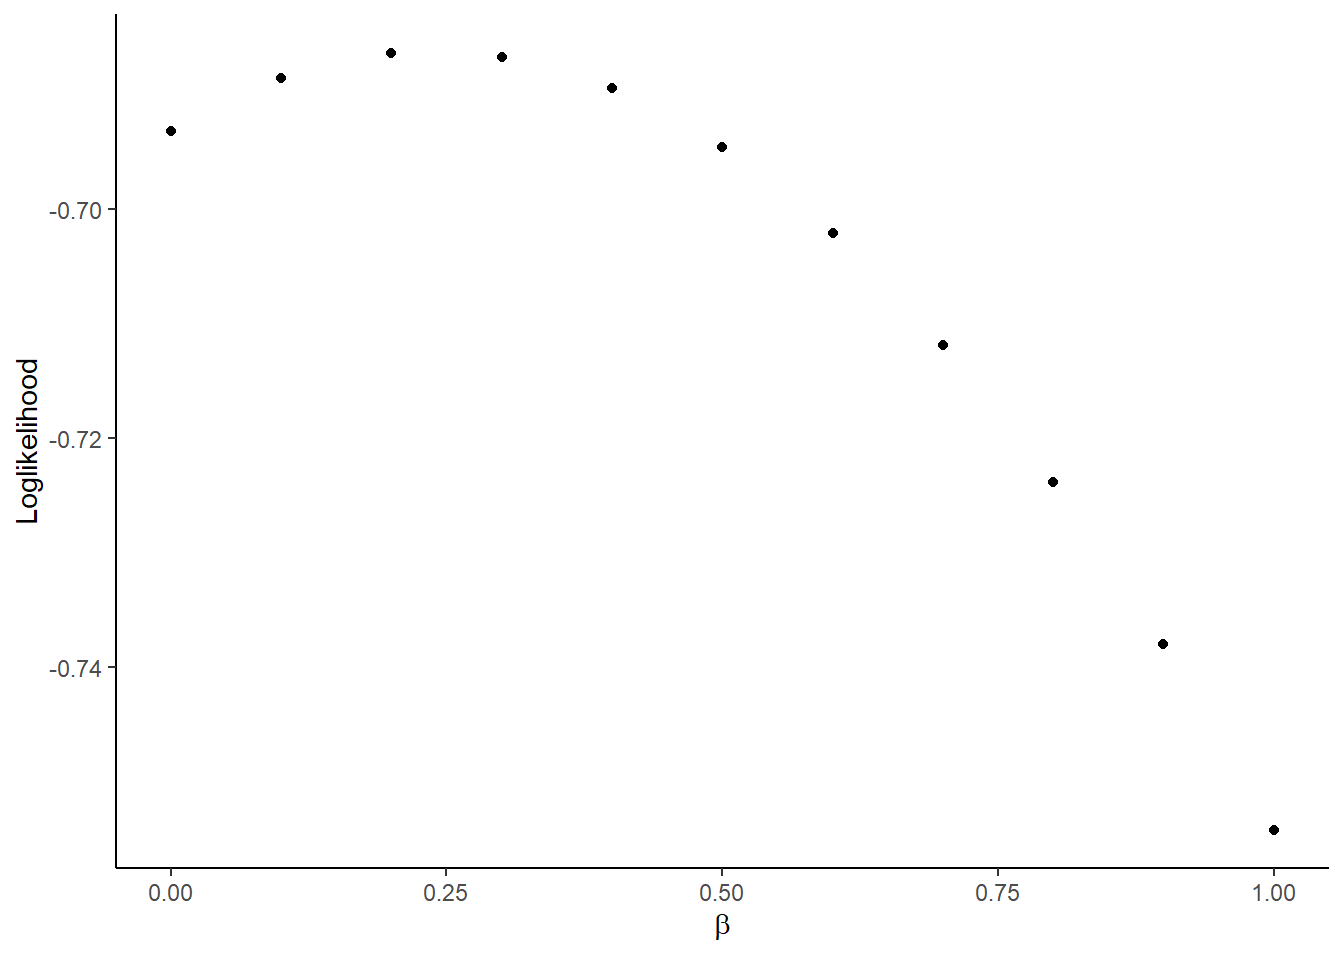
\includegraphics{6-assignment-solution_files/figure-latex/unnamed-chunk-13-1} \end{center}

\begin{verbatim}
## 
## [[2]]
\end{verbatim}

\begin{center}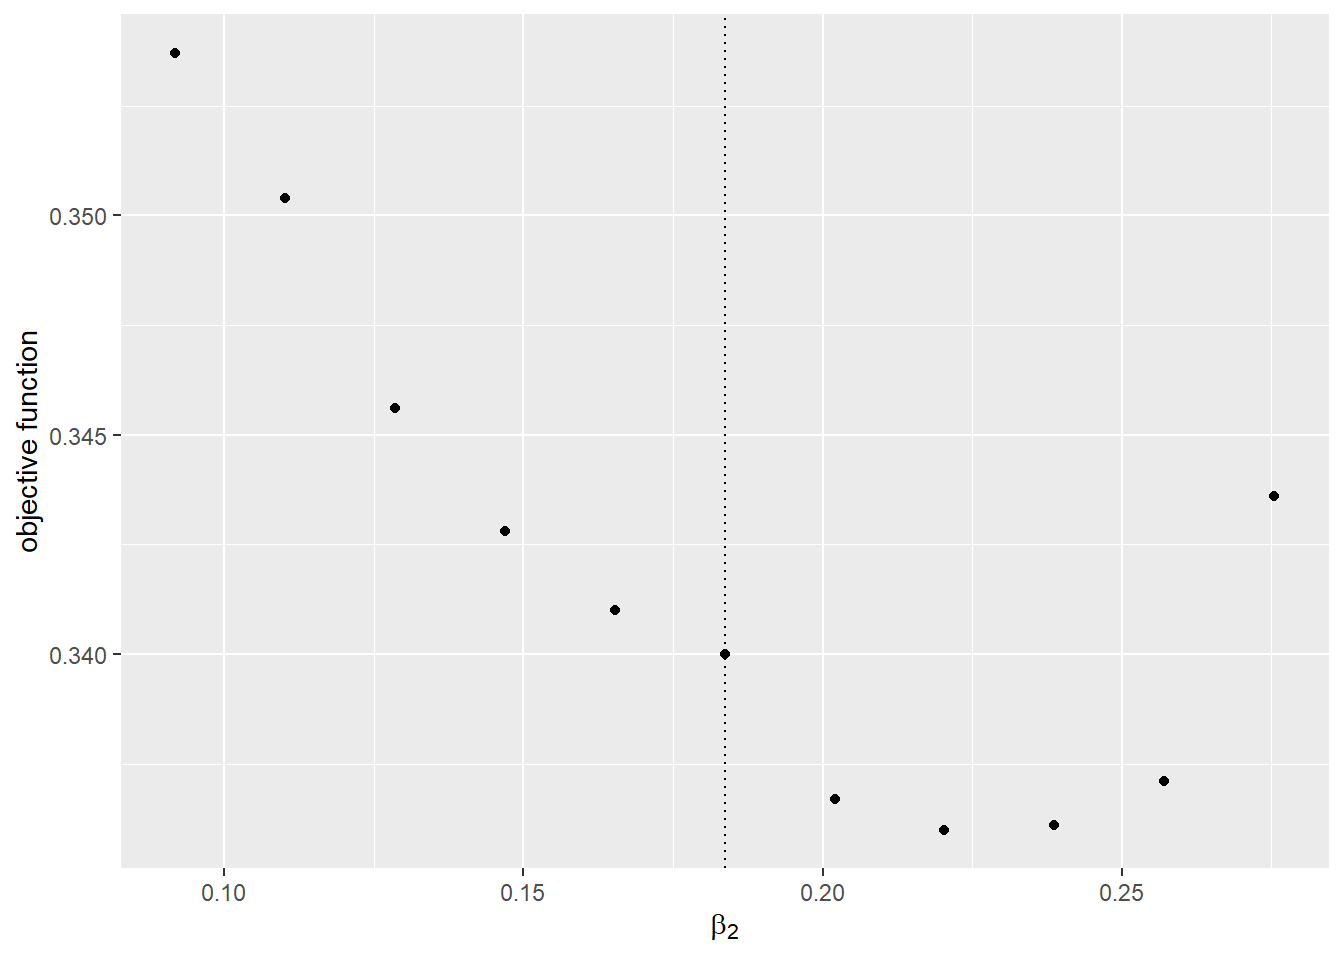
\includegraphics{6-assignment-solution_files/figure-latex/unnamed-chunk-13-2} \end{center}

\begin{verbatim}
## 
## [[3]]
\end{verbatim}

\begin{center}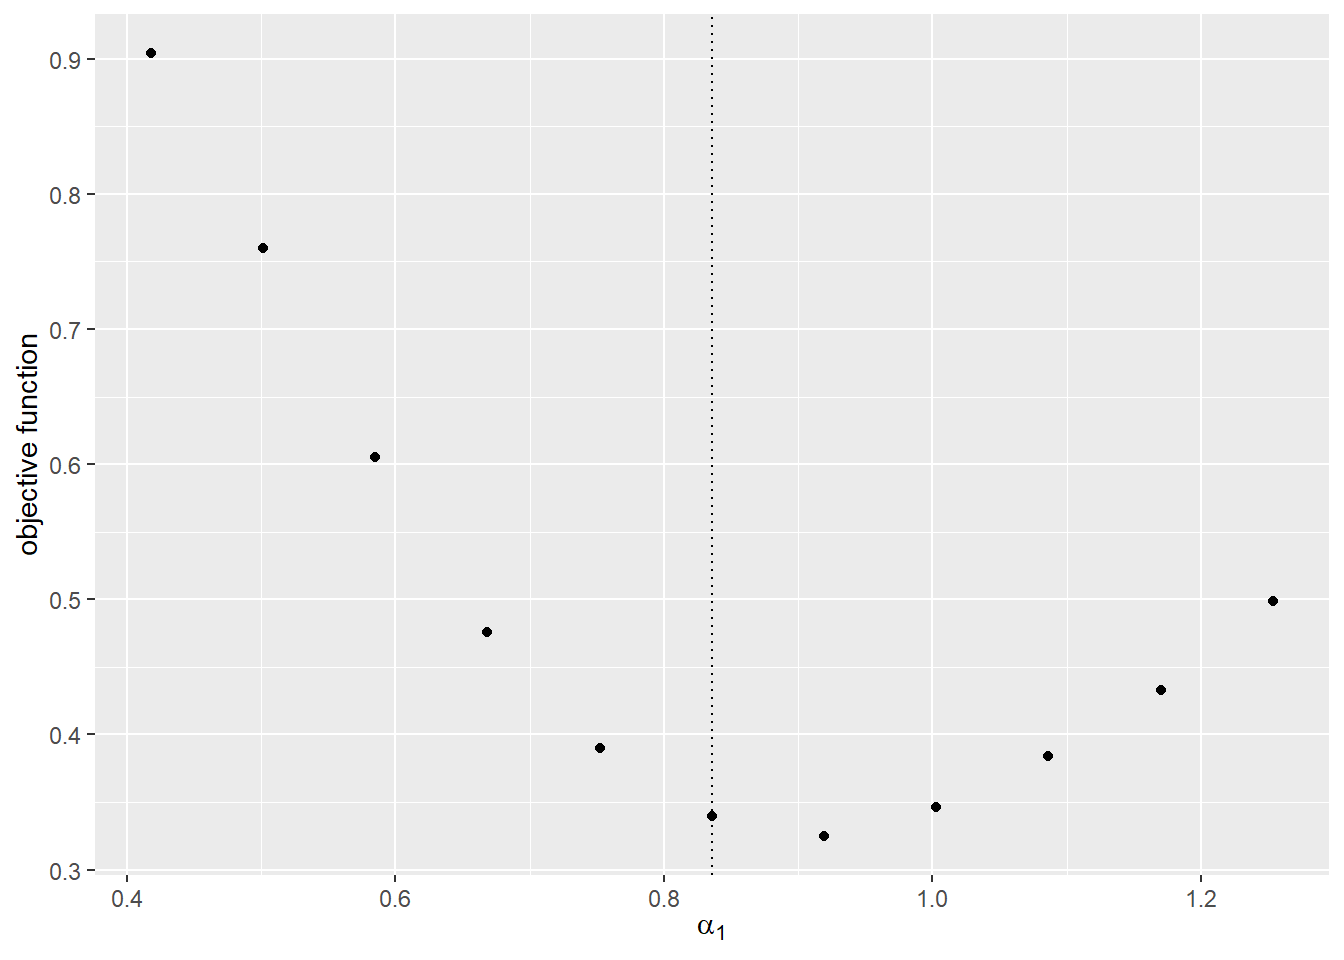
\includegraphics{6-assignment-solution_files/figure-latex/unnamed-chunk-13-3} \end{center}

\begin{verbatim}
## 
## [[4]]
\end{verbatim}

\begin{center}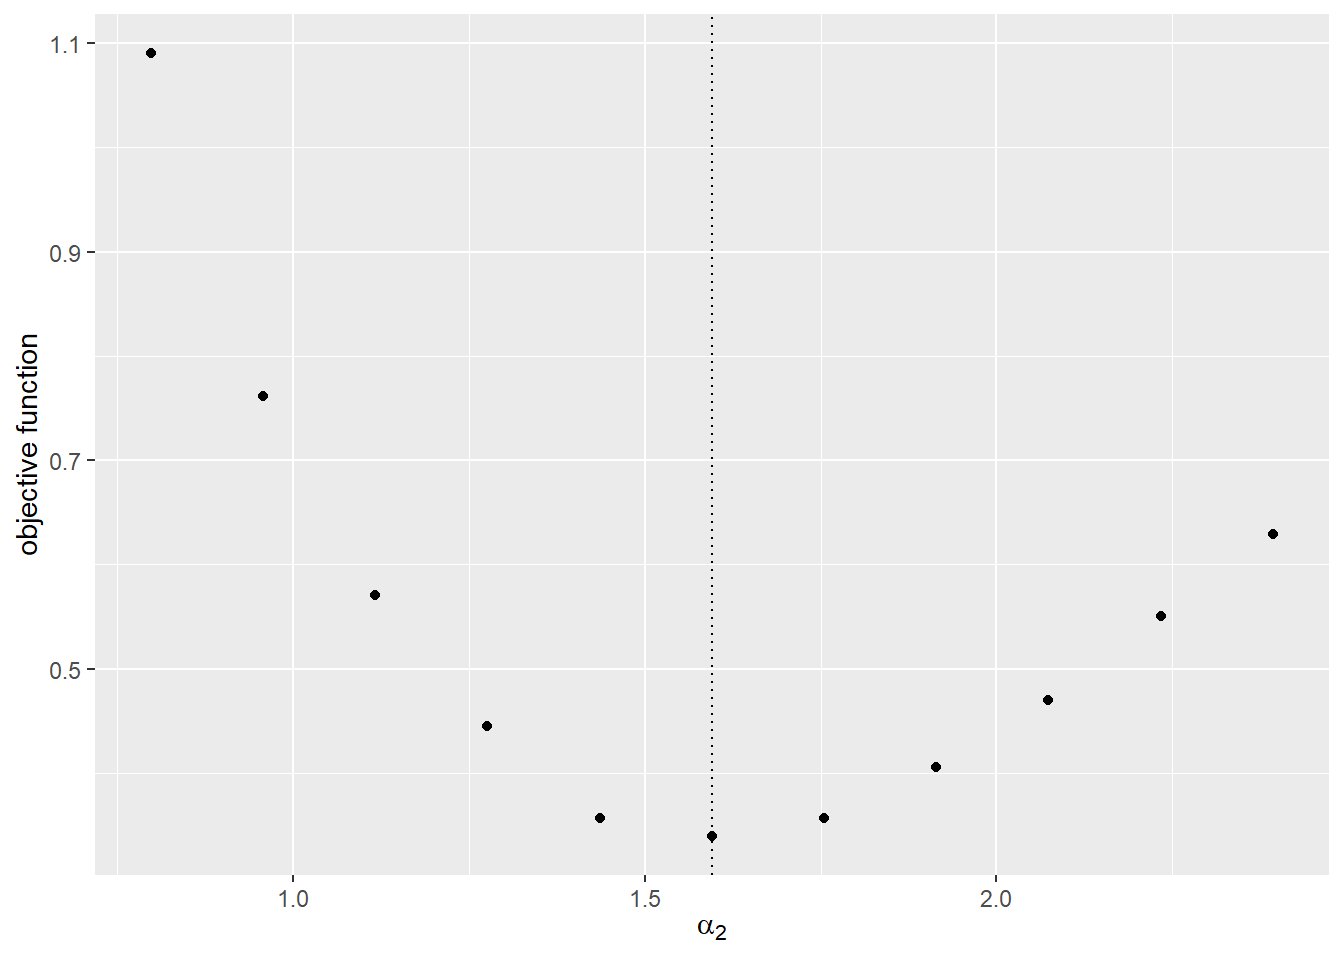
\includegraphics{6-assignment-solution_files/figure-latex/unnamed-chunk-13-4} \end{center}

\begin{verbatim}
## 
## [[5]]
\end{verbatim}

\begin{center}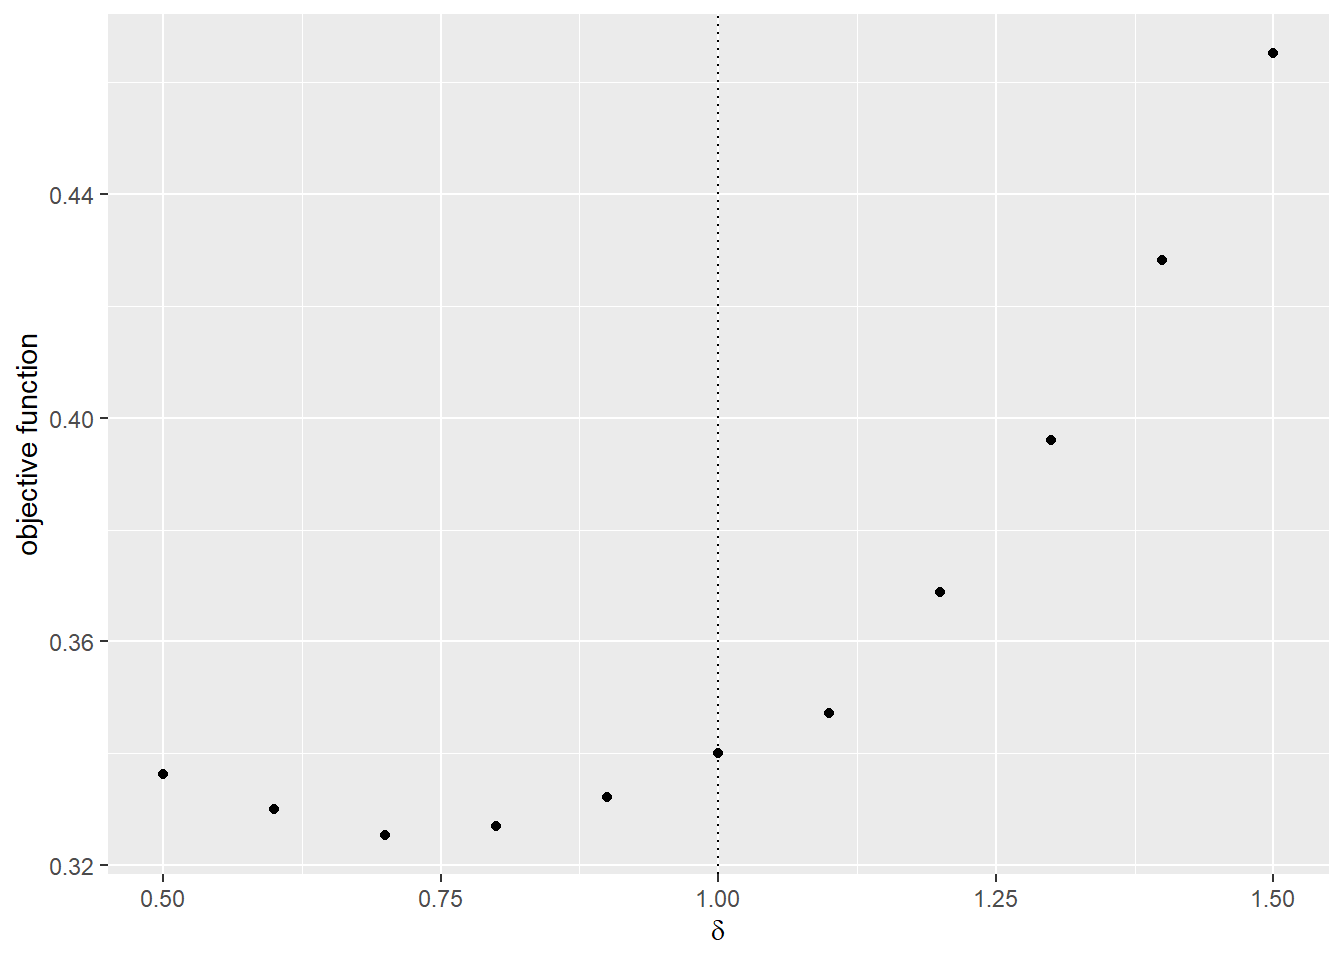
\includegraphics{6-assignment-solution_files/figure-latex/unnamed-chunk-13-5} \end{center}

\begin{verbatim}
## 
## [[6]]
\end{verbatim}

\begin{center}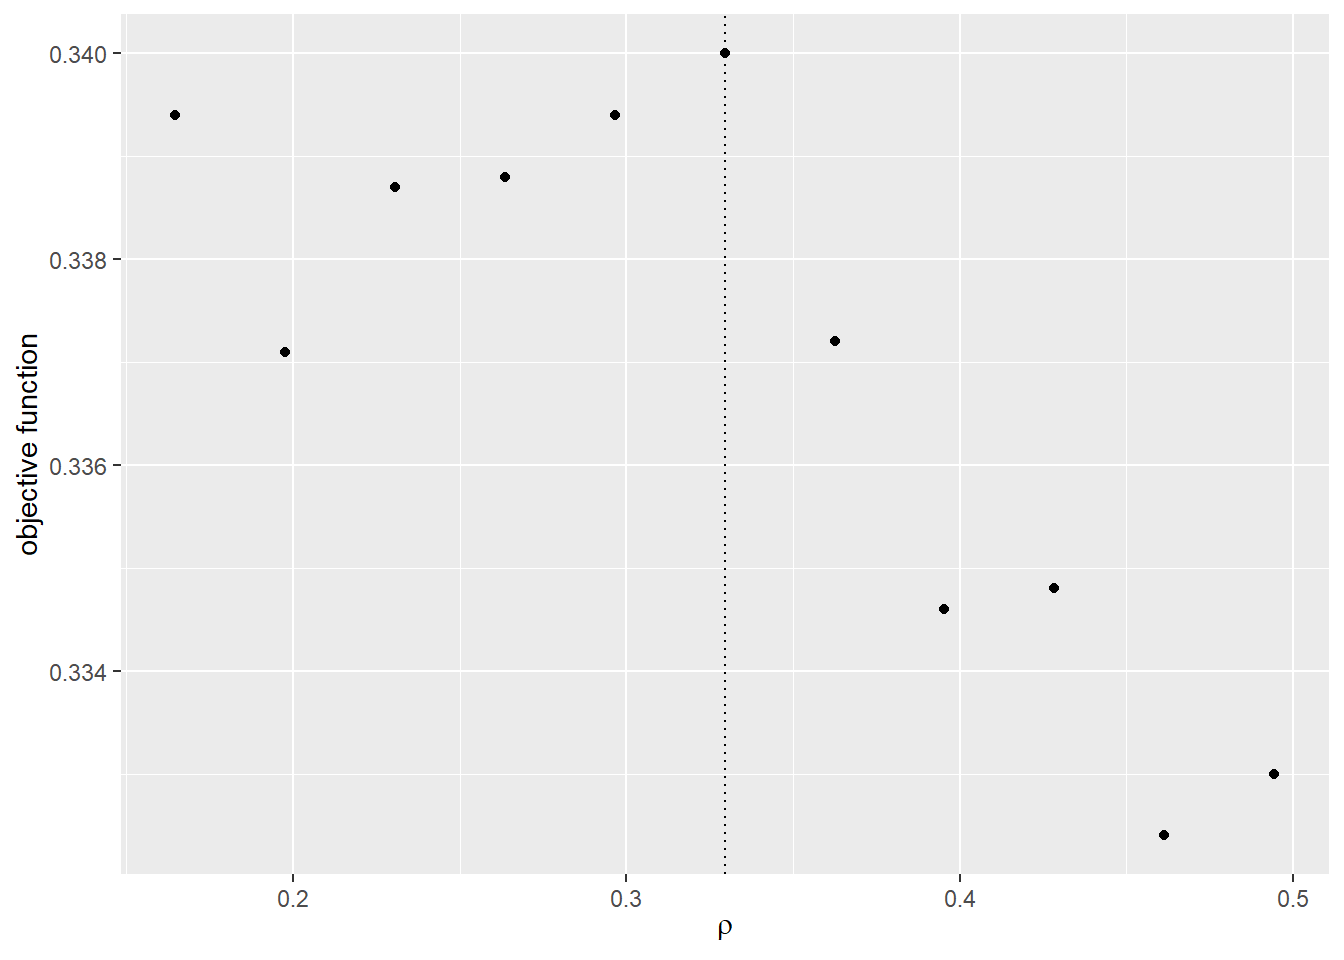
\includegraphics{6-assignment-solution_files/figure-latex/unnamed-chunk-13-6} \end{center}

\begin{enumerate}
\def\labelenumi{\arabic{enumi}.}
\setcounter{enumi}{4}
\tightlist
\item
  Check the value of the objective function around the true parameter
  under the assumption of the simultaneous entry.
\end{enumerate}

\begin{Shaded}
\begin{Highlighting}[]
\CommentTok{\# simultaneous entry}
\NormalTok{theta }\OtherTok{\textless{}{-}}\NormalTok{ theta\_simultaneous }\OtherTok{\textless{}{-}}
  \FunctionTok{c}\NormalTok{(beta, alpha, delta)}
\NormalTok{Y }\OtherTok{\textless{}{-}}\NormalTok{ Y\_simultaneous}
\NormalTok{model }\OtherTok{\textless{}{-}}\NormalTok{ compute\_simultaneous\_entry\_across\_markets}
\NormalTok{label }\OtherTok{\textless{}{-}} \FunctionTok{c}\NormalTok{(}\FunctionTok{paste}\NormalTok{(}\StringTok{"}\SpecialCharTok{\textbackslash{}\textbackslash{}}\StringTok{beta\_"}\NormalTok{, }\DecValTok{1}\SpecialCharTok{:}\NormalTok{K, }\AttributeTok{sep =} \StringTok{""}\NormalTok{), }
           \FunctionTok{paste}\NormalTok{(}\StringTok{"}\SpecialCharTok{\textbackslash{}\textbackslash{}}\StringTok{alpha\_"}\NormalTok{, }\DecValTok{1}\SpecialCharTok{:}\NormalTok{L, }\AttributeTok{sep =} \StringTok{""}\NormalTok{),}
           \StringTok{"}\SpecialCharTok{\textbackslash{}\textbackslash{}}\StringTok{delta"}\NormalTok{)}
\NormalTok{label }\OtherTok{\textless{}{-}} \FunctionTok{paste}\NormalTok{(}\StringTok{"$"}\NormalTok{, label, }\StringTok{"$"}\NormalTok{, }\AttributeTok{sep =} \StringTok{""}\NormalTok{)}
\CommentTok{\# compute the graph}
\NormalTok{graph }\OtherTok{\textless{}{-}} \FunctionTok{foreach}\NormalTok{ (}\AttributeTok{i =} \DecValTok{1}\SpecialCharTok{:}\FunctionTok{length}\NormalTok{(theta)) }\SpecialCharTok{\%do\%}\NormalTok{ \{}
\NormalTok{  theta\_i }\OtherTok{\textless{}{-}}\NormalTok{ theta[i]}
\NormalTok{  theta\_i\_list }\OtherTok{\textless{}{-}}\NormalTok{ theta\_i }\SpecialCharTok{*} \FunctionTok{seq}\NormalTok{(}\FloatTok{0.5}\NormalTok{, }\FloatTok{1.5}\NormalTok{, }\AttributeTok{by =} \FloatTok{0.1}\NormalTok{)}
\NormalTok{  objective\_i }\OtherTok{\textless{}{-}} 
    \FunctionTok{foreach}\NormalTok{ (}\AttributeTok{j =} \DecValTok{1}\SpecialCharTok{:}\FunctionTok{length}\NormalTok{(theta\_i\_list),}
             \AttributeTok{.combine =} \StringTok{"rbind"}\NormalTok{) }\SpecialCharTok{\%do\%}\NormalTok{ \{}
\NormalTok{               theta\_ij }\OtherTok{\textless{}{-}}\NormalTok{ theta\_i\_list[j]}
\NormalTok{               theta\_j }\OtherTok{\textless{}{-}}\NormalTok{ theta}
\NormalTok{               theta\_j[i] }\OtherTok{\textless{}{-}}\NormalTok{ theta\_ij}
\NormalTok{               objective\_ij }\OtherTok{\textless{}{-}} 
                 \FunctionTok{compute\_objective\_simultaneous\_entry}\NormalTok{(Y, X, Z, EP\_mc, NU\_mc, theta\_j)}
               \FunctionTok{return}\NormalTok{(objective\_ij)}
\NormalTok{             \}}
\NormalTok{  df\_graph }\OtherTok{\textless{}{-}} \FunctionTok{data.frame}\NormalTok{(}\AttributeTok{x =}\NormalTok{ theta\_i\_list, }\AttributeTok{y =}\NormalTok{ objective\_i) }
\NormalTok{  g }\OtherTok{\textless{}{-}} \FunctionTok{ggplot}\NormalTok{(}\AttributeTok{data =}\NormalTok{ df\_graph, }\FunctionTok{aes}\NormalTok{(}\AttributeTok{x =}\NormalTok{ x, }\AttributeTok{y =}\NormalTok{ y)) }\SpecialCharTok{+} 
    \FunctionTok{geom\_point}\NormalTok{() }\SpecialCharTok{+}
    \FunctionTok{geom\_vline}\NormalTok{(}\AttributeTok{xintercept =}\NormalTok{ theta\_i, }\AttributeTok{linetype =} \StringTok{"dotted"}\NormalTok{) }\SpecialCharTok{+}
    \FunctionTok{ylab}\NormalTok{(}\StringTok{"objective function"}\NormalTok{) }\SpecialCharTok{+} \FunctionTok{xlab}\NormalTok{(}\FunctionTok{TeX}\NormalTok{(label[i]))}
  \FunctionTok{return}\NormalTok{(g)}
\NormalTok{\}}
\FunctionTok{save}\NormalTok{(graph, }\AttributeTok{file =} \StringTok{"data/A6\_graph\_simultaneous.RData"}\NormalTok{)}
\end{Highlighting}
\end{Shaded}

\begin{Shaded}
\begin{Highlighting}[]
\FunctionTok{load}\NormalTok{(}\AttributeTok{file =} \StringTok{"data/A6\_graph\_simultaneous.RData"}\NormalTok{)}
\NormalTok{graph}
\end{Highlighting}
\end{Shaded}

\begin{verbatim}
## [[1]]
\end{verbatim}

\begin{center}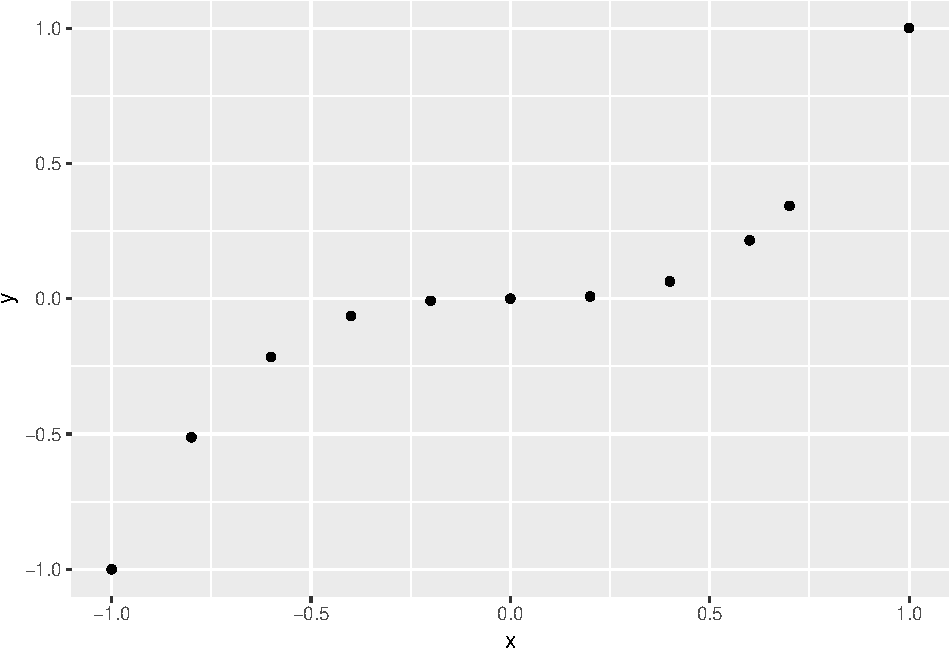
\includegraphics{6-assignment-solution_files/figure-latex/unnamed-chunk-15-1} \end{center}

\begin{verbatim}
## 
## [[2]]
\end{verbatim}

\begin{center}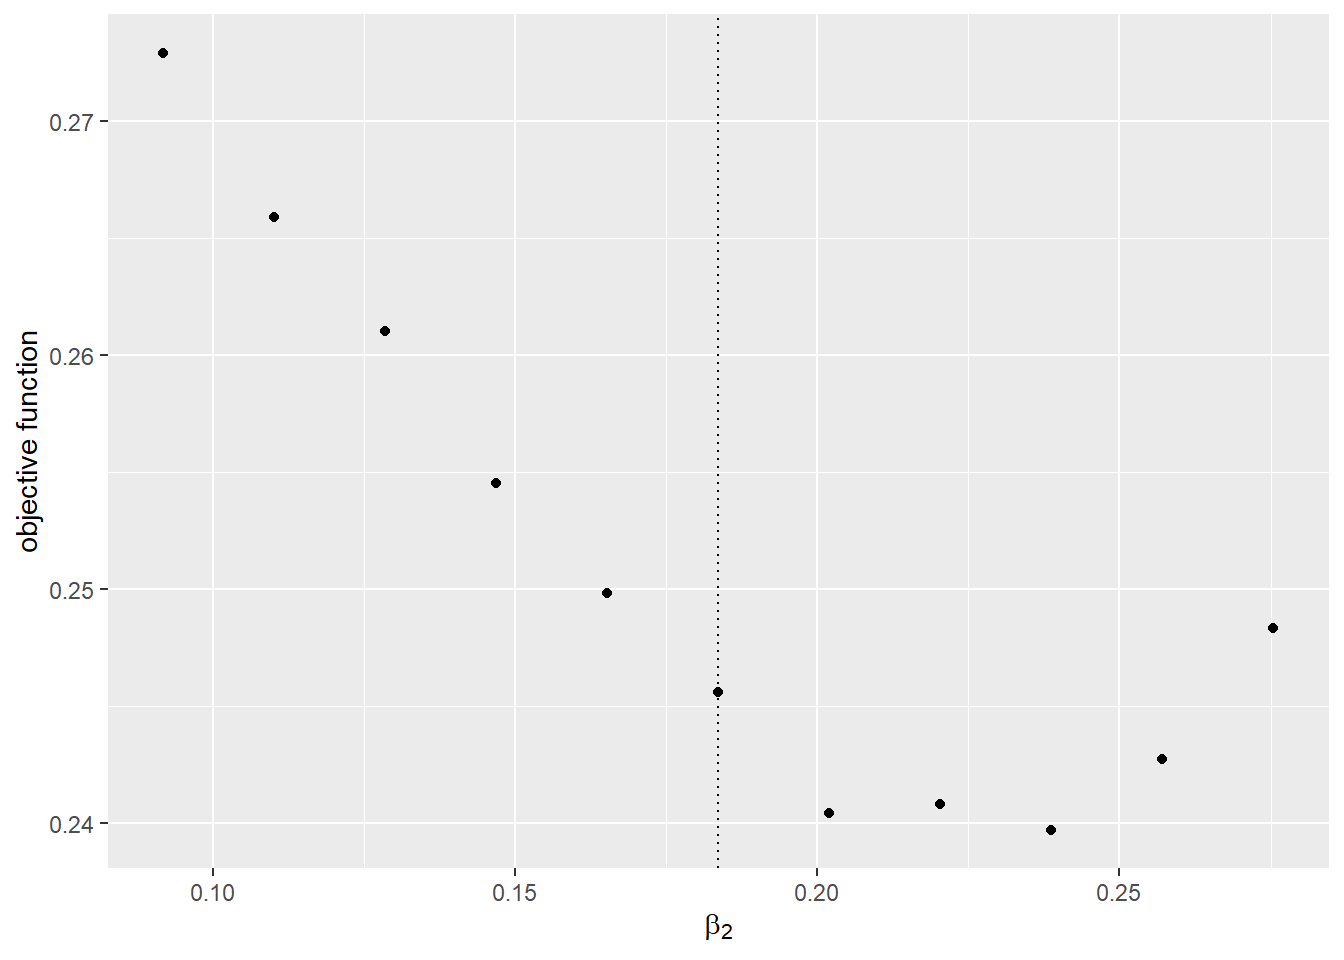
\includegraphics{6-assignment-solution_files/figure-latex/unnamed-chunk-15-2} \end{center}

\begin{verbatim}
## 
## [[3]]
\end{verbatim}

\begin{center}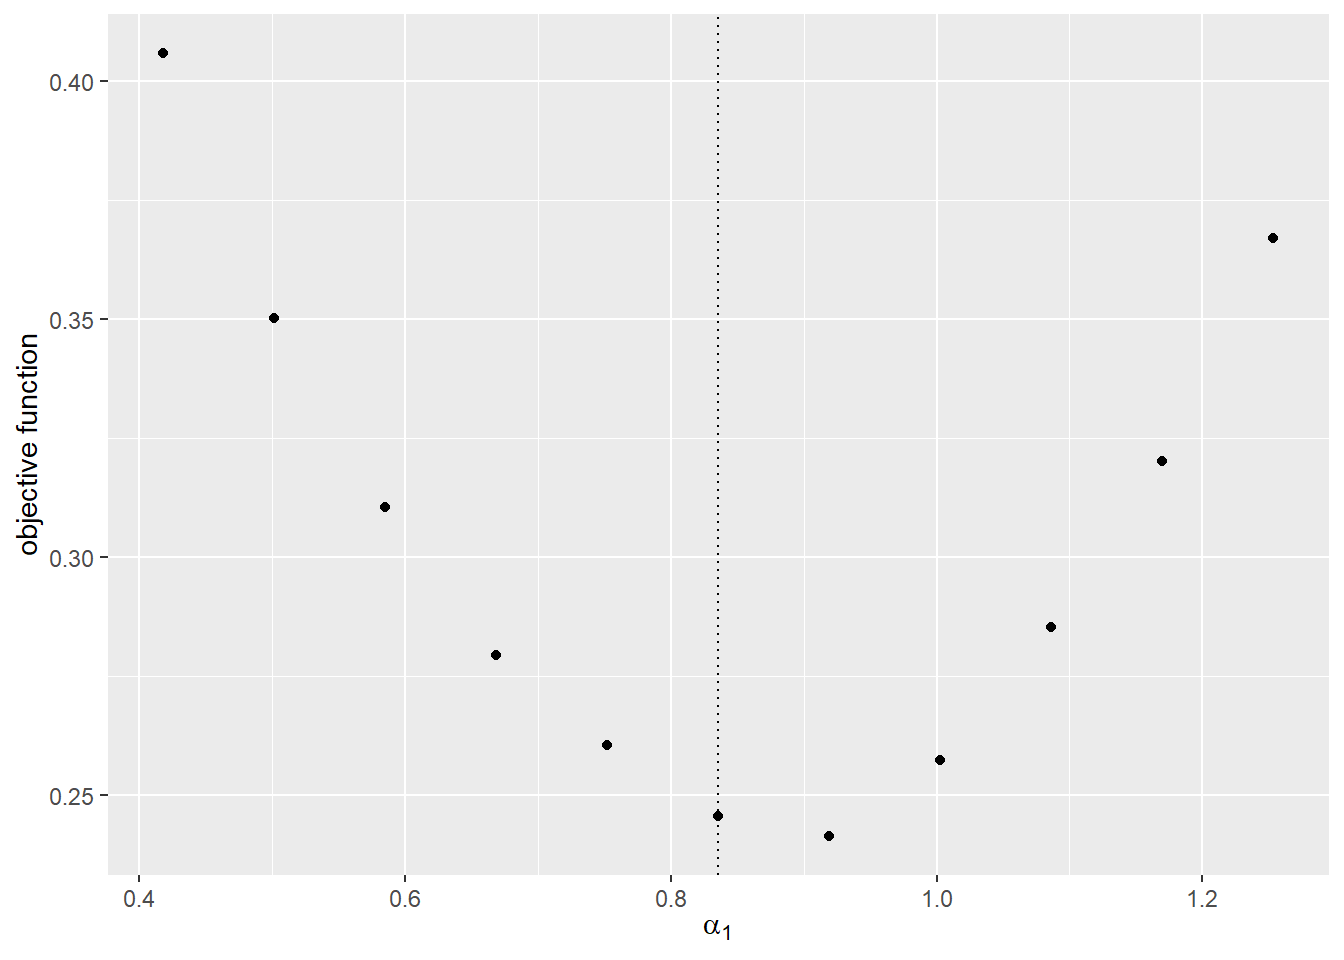
\includegraphics{6-assignment-solution_files/figure-latex/unnamed-chunk-15-3} \end{center}

\begin{verbatim}
## 
## [[4]]
\end{verbatim}

\begin{center}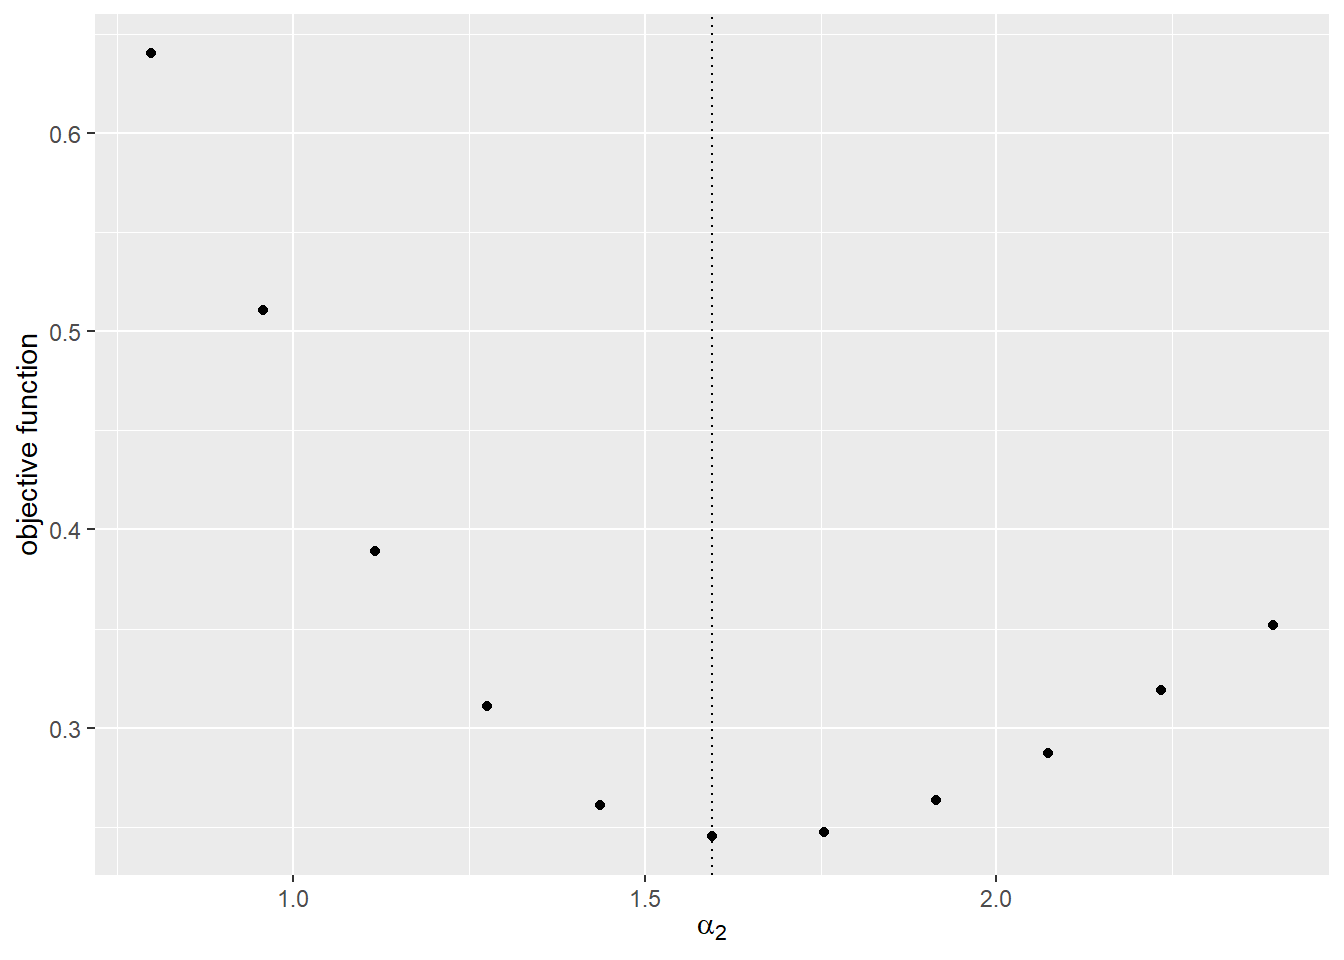
\includegraphics{6-assignment-solution_files/figure-latex/unnamed-chunk-15-4} \end{center}

\begin{verbatim}
## 
## [[5]]
\end{verbatim}

\begin{center}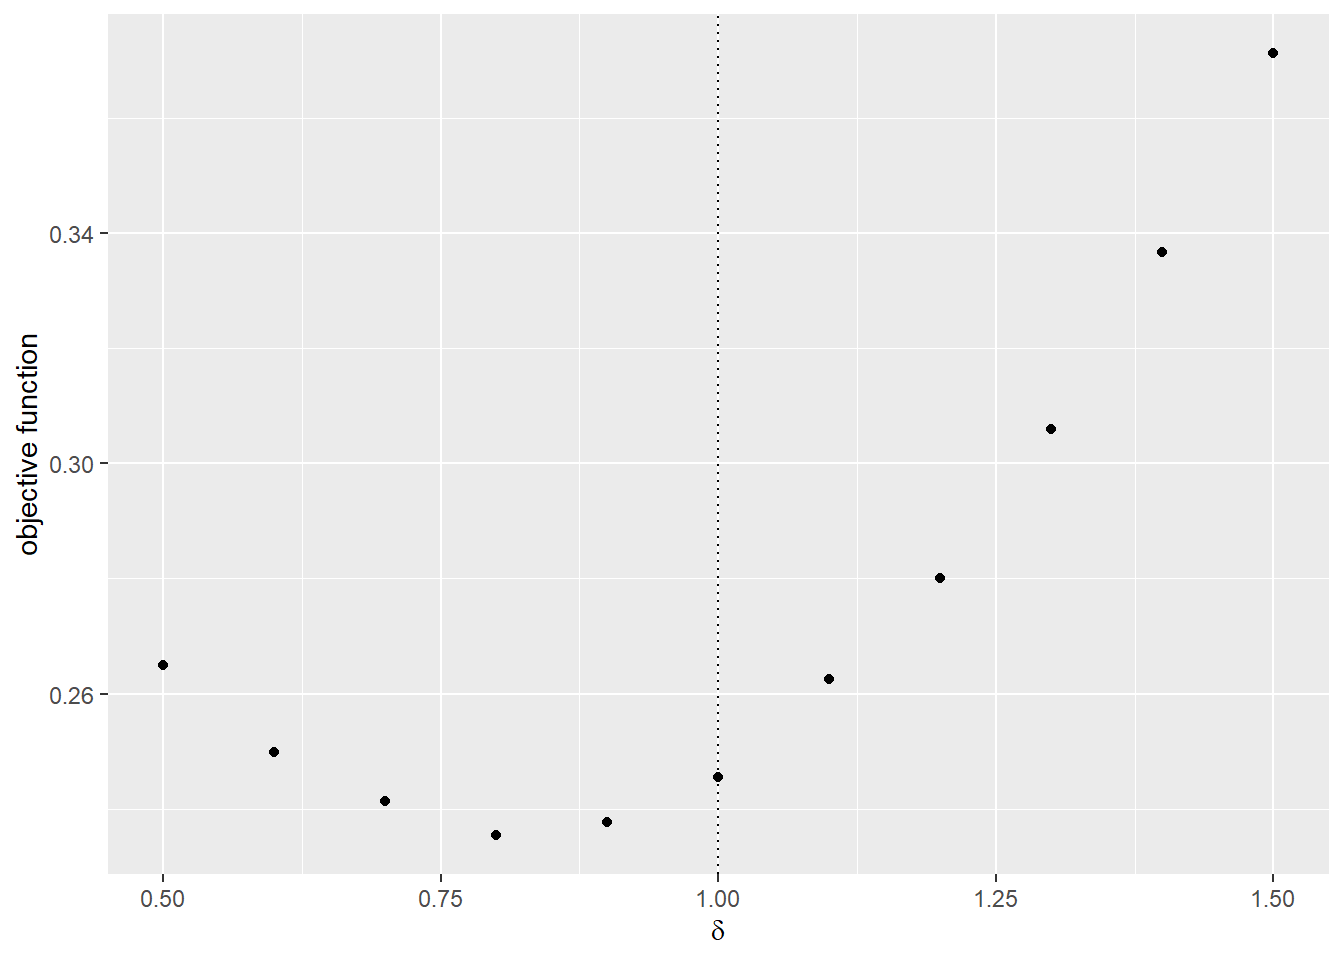
\includegraphics{6-assignment-solution_files/figure-latex/unnamed-chunk-15-5} \end{center}

\begin{enumerate}
\def\labelenumi{\arabic{enumi}.}
\setcounter{enumi}{5}
\tightlist
\item
  Estimate the parameters under the assumption of the sequential entry.
\end{enumerate}

\begin{Shaded}
\begin{Highlighting}[]
\CommentTok{\# sequential entry}
\NormalTok{theta }\OtherTok{\textless{}{-}}\NormalTok{ theta\_sequential }\OtherTok{\textless{}{-}}
  \FunctionTok{c}\NormalTok{(beta, alpha, delta, rho)}
\end{Highlighting}
\end{Shaded}

\begin{Shaded}
\begin{Highlighting}[]
\NormalTok{Y }\OtherTok{\textless{}{-}}\NormalTok{ Y\_sequential}
\NormalTok{result\_sequential }\OtherTok{\textless{}{-}}
  \FunctionTok{optim}\NormalTok{(}\AttributeTok{par =}\NormalTok{ theta,}
        \AttributeTok{fn =}\NormalTok{ compute\_objective\_sequential\_entry,}
        \AttributeTok{method =} \StringTok{"Nelder{-}Mead"}\NormalTok{,}
        \AttributeTok{Y =}\NormalTok{ Y,}
        \AttributeTok{X =}\NormalTok{ X,}
        \AttributeTok{Z =}\NormalTok{ Z,}
        \AttributeTok{EP\_mc =}\NormalTok{ EP\_mc,}
        \AttributeTok{NU\_mc =}\NormalTok{ NU\_mc)}
\FunctionTok{save}\NormalTok{(result\_sequential, }\AttributeTok{file =} \StringTok{"data/A6\_estimate\_sequential.RData"}\NormalTok{)}
\end{Highlighting}
\end{Shaded}

\begin{Shaded}
\begin{Highlighting}[]
\FunctionTok{load}\NormalTok{(}\AttributeTok{file =} \StringTok{"data/A6\_estimate\_sequential.RData"}\NormalTok{)}
\NormalTok{result\_sequential}
\end{Highlighting}
\end{Shaded}

\begin{verbatim}
## $par
## [1] 0.59704343 0.04938142 0.93904853 1.80598524 1.04483638 0.39060511
## 
## $value
## [1] 0.2762
## 
## $counts
## function gradient 
##      155       NA 
## 
## $convergence
## [1] 0
## 
## $message
## NULL
\end{verbatim}

\begin{Shaded}
\begin{Highlighting}[]
\NormalTok{comparison }\OtherTok{\textless{}{-}}
  \FunctionTok{data.frame}\NormalTok{(}
    \AttributeTok{actual =}\NormalTok{ theta,}
    \AttributeTok{estimate =}\NormalTok{ result\_sequential}\SpecialCharTok{$}\NormalTok{par}
\NormalTok{  )}
\NormalTok{comparison}
\end{Highlighting}
\end{Shaded}

\begin{verbatim}
##      actual   estimate
## 1 0.6264538 0.59704343
## 2 0.1836433 0.04938142
## 3 0.8356286 0.93904853
## 4 1.5952808 1.80598524
## 5 1.0000000 1.04483638
## 6 0.3295078 0.39060511
\end{verbatim}

\begin{enumerate}
\def\labelenumi{\arabic{enumi}.}
\setcounter{enumi}{6}
\tightlist
\item
  Estimate the parameters under the assumption of the simultaneous
  entry. Set the lower bound for \(\delta\) at 0.
\end{enumerate}

\begin{Shaded}
\begin{Highlighting}[]
\CommentTok{\# simultaneous entry}
\NormalTok{theta }\OtherTok{\textless{}{-}}\NormalTok{ theta\_simultaneous }\OtherTok{\textless{}{-}}
  \FunctionTok{c}\NormalTok{(beta, alpha, delta, rho)}
\end{Highlighting}
\end{Shaded}

\begin{Shaded}
\begin{Highlighting}[]
\NormalTok{Y }\OtherTok{\textless{}{-}}\NormalTok{ Y\_sequential}
\NormalTok{result\_simultaneous }\OtherTok{\textless{}{-}}
  \FunctionTok{optim}\NormalTok{(}\AttributeTok{par =}\NormalTok{ theta,}
        \AttributeTok{fn =}\NormalTok{ compute\_objective\_simultaneous\_entry,}
        \AttributeTok{method =} \StringTok{"Nelder{-}Mead"}\NormalTok{,}
        \AttributeTok{Y =}\NormalTok{ Y,}
        \AttributeTok{X =}\NormalTok{ X,}
        \AttributeTok{Z =}\NormalTok{ Z,}
        \AttributeTok{EP\_mc =}\NormalTok{ EP\_mc,}
        \AttributeTok{NU\_mc =}\NormalTok{ NU\_mc)}
\FunctionTok{save}\NormalTok{(result\_simultaneous, }\AttributeTok{file =} \StringTok{"data/A6\_estimate\_simultaneous.RData"}\NormalTok{)}
\end{Highlighting}
\end{Shaded}

\begin{Shaded}
\begin{Highlighting}[]
\FunctionTok{load}\NormalTok{(}\AttributeTok{file =} \StringTok{"data/A6\_estimate\_simultaneous.RData"}\NormalTok{)}
\NormalTok{result\_simultaneous}
\end{Highlighting}
\end{Shaded}

\begin{verbatim}
## $par
## [1] 0.5787563 0.1216856 0.9521359 1.8443535 1.2177670 0.3075741
## 
## $value
## [1] 0.1623
## 
## $counts
## function gradient 
##      141       NA 
## 
## $convergence
## [1] 0
## 
## $message
## NULL
\end{verbatim}

\begin{Shaded}
\begin{Highlighting}[]
\NormalTok{comparison }\OtherTok{\textless{}{-}}
  \FunctionTok{data.frame}\NormalTok{(}
    \AttributeTok{actual =}\NormalTok{ theta,}
    \AttributeTok{estimate =}\NormalTok{ result\_simultaneous}\SpecialCharTok{$}\NormalTok{par}
\NormalTok{  )}
\NormalTok{comparison}
\end{Highlighting}
\end{Shaded}

\begin{verbatim}
##      actual  estimate
## 1 0.6264538 0.5787563
## 2 0.1836433 0.1216856
## 3 0.8356286 0.9521359
## 4 1.5952808 1.8443535
## 5 1.0000000 1.2177670
## 6 0.3295078 0.3075741
\end{verbatim}

\hypertarget{conduct-counterfactual-simulations}{%
\subsection{Conduct counterfactual
simulations}\label{conduct-counterfactual-simulations}}

\begin{enumerate}
\def\labelenumi{\arabic{enumi}.}
\tightlist
\item
  Fix the first draw of the Monte Carlo shocks. Suppose that the
  competitive effect becomes mild, i.e.~\(\delta\) is changed to 0.5.
  Under these shocks, compute the equilibrium number of entrants across
  markets and plot the histogram with the estimated and counterfactual
  parameters. Conduct this analysis under the assumptions of sequential
  and simultaneous entry.
\end{enumerate}

\begin{Shaded}
\begin{Highlighting}[]
\CommentTok{\# sequential entry}
\CommentTok{\# extract parameters}
\NormalTok{theta }\OtherTok{\textless{}{-}}\NormalTok{ result\_sequential}\SpecialCharTok{$}\NormalTok{par}
\NormalTok{K }\OtherTok{\textless{}{-}} \FunctionTok{dim}\NormalTok{(X)[}\DecValTok{2}\NormalTok{]}
\NormalTok{L }\OtherTok{\textless{}{-}} \FunctionTok{dim}\NormalTok{(Z[[}\DecValTok{1}\NormalTok{]])[}\DecValTok{2}\NormalTok{]}
\NormalTok{beta }\OtherTok{\textless{}{-}}\NormalTok{ theta[}\DecValTok{1}\SpecialCharTok{:}\NormalTok{K]}
\NormalTok{alpha }\OtherTok{\textless{}{-}}\NormalTok{ theta[(K }\SpecialCharTok{+} \DecValTok{1}\NormalTok{)}\SpecialCharTok{:}\NormalTok{(K }\SpecialCharTok{+}\NormalTok{ L)]}
\NormalTok{delta }\OtherTok{\textless{}{-}}\NormalTok{ theta[K }\SpecialCharTok{+}\NormalTok{ L }\SpecialCharTok{+} \DecValTok{1}\NormalTok{]}
\NormalTok{rho }\OtherTok{\textless{}{-}}\NormalTok{ theta[K }\SpecialCharTok{+}\NormalTok{ L }\SpecialCharTok{+} \DecValTok{2}\NormalTok{]}
\CommentTok{\# monte carlo simulations under the actual parameters}
\NormalTok{Y\_actual }\OtherTok{\textless{}{-}} 
  \FunctionTok{compute\_monte\_carlo\_sequential\_entry}\NormalTok{(}
\NormalTok{    X, Z, EP\_mc[}\DecValTok{1}\NormalTok{], NU\_mc[}\DecValTok{1}\NormalTok{], beta, alpha, delta, rho)}
\NormalTok{Y\_actual }\OtherTok{\textless{}{-}}\NormalTok{ Y\_actual[[}\DecValTok{1}\NormalTok{]]}
\CommentTok{\# monte carlo simulations under the counterfactual parameters}
\NormalTok{delta\_count }\OtherTok{\textless{}{-}} \FloatTok{0.5}
\NormalTok{Y\_count }\OtherTok{\textless{}{-}} 
  \FunctionTok{compute\_monte\_carlo\_sequential\_entry}\NormalTok{(}
\NormalTok{    X, Z, EP\_mc[}\DecValTok{1}\NormalTok{], NU\_mc[}\DecValTok{1}\NormalTok{], beta, alpha, delta\_count, rho)}
\NormalTok{Y\_count }\OtherTok{\textless{}{-}}\NormalTok{ Y\_count[[}\DecValTok{1}\NormalTok{]]}
\CommentTok{\# histogram}
\NormalTok{N\_actual }\OtherTok{\textless{}{-}}
\NormalTok{  Y\_actual }\SpecialCharTok{\%\textgreater{}\%}
\NormalTok{  purrr}\SpecialCharTok{::}\FunctionTok{map}\NormalTok{(sum) }\SpecialCharTok{\%\textgreater{}\%}
\NormalTok{  purrr}\SpecialCharTok{::}\FunctionTok{reduce}\NormalTok{(rbind) }\SpecialCharTok{\%\textgreater{}\%}
  \FunctionTok{as.integer}\NormalTok{()}
\NormalTok{N\_count }\OtherTok{\textless{}{-}}
\NormalTok{  Y\_count }\SpecialCharTok{\%\textgreater{}\%}
\NormalTok{  purrr}\SpecialCharTok{::}\FunctionTok{map}\NormalTok{(sum) }\SpecialCharTok{\%\textgreater{}\%}
\NormalTok{  purrr}\SpecialCharTok{::}\FunctionTok{reduce}\NormalTok{(rbind) }\SpecialCharTok{\%\textgreater{}\%}
  \FunctionTok{as.integer}\NormalTok{()}
\NormalTok{N\_df }\OtherTok{\textless{}{-}} \FunctionTok{data.frame}\NormalTok{(}
  \AttributeTok{m =} \DecValTok{1}\SpecialCharTok{:}\FunctionTok{length}\NormalTok{(N\_actual),}
  \AttributeTok{actual =}\NormalTok{ N\_actual,}
  \AttributeTok{count =}\NormalTok{ N\_count}
\NormalTok{) }\SpecialCharTok{\%\textgreater{}\%}
\NormalTok{  reshape2}\SpecialCharTok{::}\FunctionTok{melt}\NormalTok{(}\AttributeTok{id.vars =} \StringTok{"m"}\NormalTok{) }\SpecialCharTok{\%\textgreater{}\%}
\NormalTok{  dplyr}\SpecialCharTok{::}\FunctionTok{rename}\NormalTok{(}\AttributeTok{parameters =}\NormalTok{ variable) }\SpecialCharTok{\%\textgreater{}\%}
\NormalTok{  dplyr}\SpecialCharTok{::}\FunctionTok{group\_by}\NormalTok{(parameters, value) }\SpecialCharTok{\%\textgreater{}\%}
\NormalTok{  dplyr}\SpecialCharTok{::}\FunctionTok{summarise}\NormalTok{(}\AttributeTok{n =} \FunctionTok{length}\NormalTok{(m)) }\SpecialCharTok{\%\textgreater{}\%}
\NormalTok{  dplyr}\SpecialCharTok{::}\FunctionTok{ungroup}\NormalTok{() }\SpecialCharTok{\%\textgreater{}\%}
\NormalTok{  tidyr}\SpecialCharTok{::}\FunctionTok{complete}\NormalTok{(parameters, value, }\AttributeTok{fill =} \FunctionTok{list}\NormalTok{(}\AttributeTok{n =} \DecValTok{0}\NormalTok{))}
\end{Highlighting}
\end{Shaded}

\begin{verbatim}
## `summarise()` regrouping output by 'parameters' (override with `.groups` argument)
\end{verbatim}

\begin{Shaded}
\begin{Highlighting}[]
\FunctionTok{ggplot}\NormalTok{(N\_df, }\FunctionTok{aes}\NormalTok{(}\AttributeTok{x =}\NormalTok{ value, }\AttributeTok{y =}\NormalTok{ n, }\AttributeTok{colour =}\NormalTok{ parameters, }\AttributeTok{fill =}\NormalTok{ parameters)) }\SpecialCharTok{+}
  \FunctionTok{geom\_bar}\NormalTok{(}\AttributeTok{stat =} \StringTok{"identity"}\NormalTok{, }\AttributeTok{position =} \StringTok{"dodge"}\NormalTok{) }\SpecialCharTok{+}
  \FunctionTok{ylab}\NormalTok{(}\StringTok{"count"}\NormalTok{) }\SpecialCharTok{+} \FunctionTok{xlab}\NormalTok{(}\StringTok{"number of entrants"}\NormalTok{) }\SpecialCharTok{+} \FunctionTok{ggtitle}\NormalTok{(}\StringTok{"Sequential entry"}\NormalTok{) }\SpecialCharTok{+}
  \FunctionTok{theme}\NormalTok{(}\AttributeTok{plot.title =} \FunctionTok{element\_text}\NormalTok{(}\AttributeTok{hjust =} \FloatTok{0.5}\NormalTok{))}
\end{Highlighting}
\end{Shaded}

\begin{center}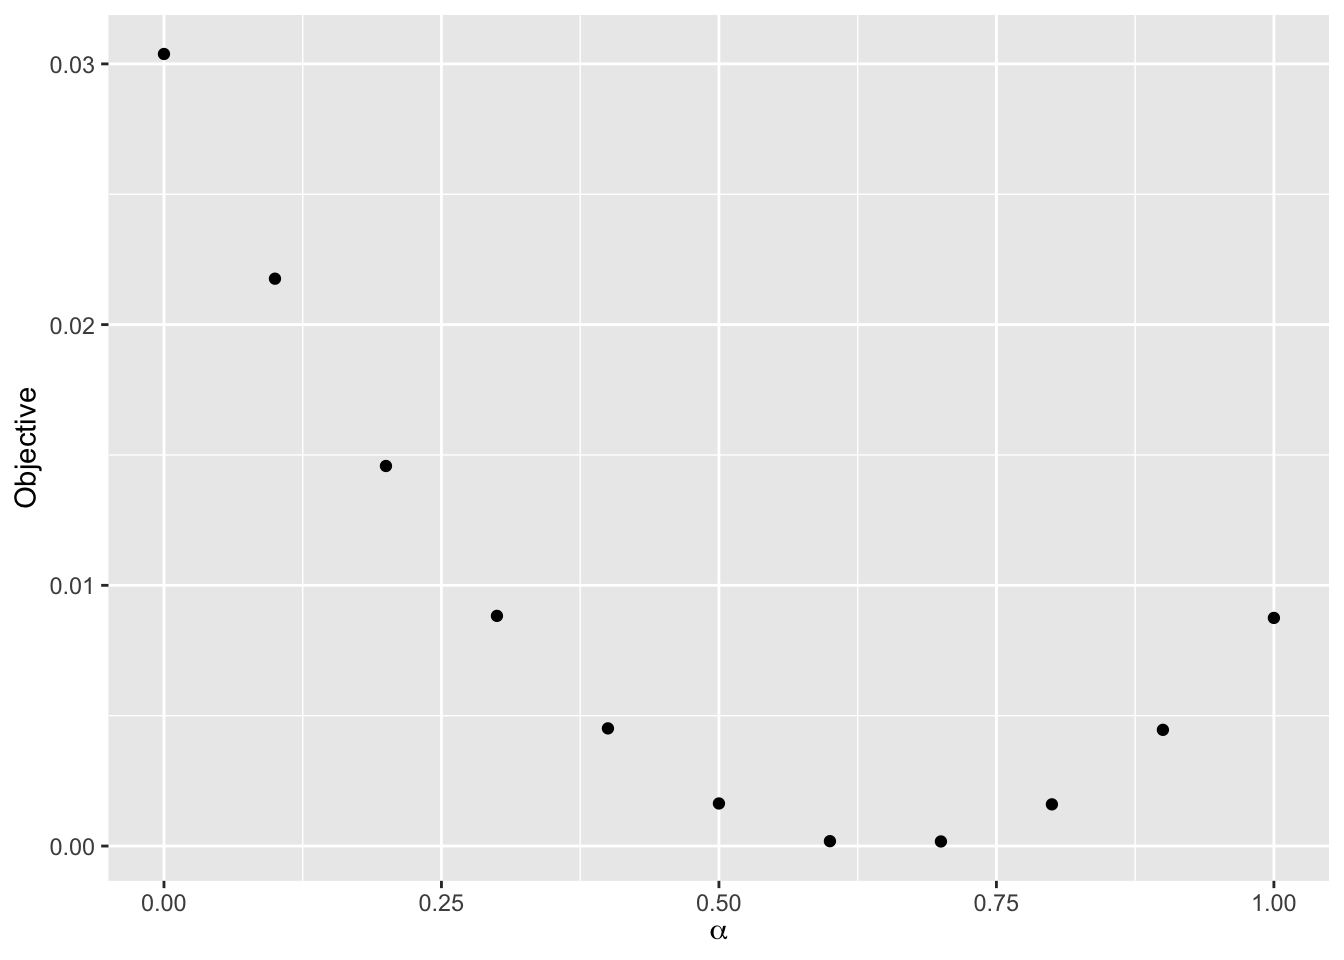
\includegraphics{6-assignment-solution_files/figure-latex/unnamed-chunk-22-1} \end{center}

\begin{Shaded}
\begin{Highlighting}[]
\CommentTok{\# simultaneous entry}
\CommentTok{\# extract parameters}
\NormalTok{theta }\OtherTok{\textless{}{-}}\NormalTok{ result\_simultaneous}\SpecialCharTok{$}\NormalTok{par}
\NormalTok{K }\OtherTok{\textless{}{-}} \FunctionTok{dim}\NormalTok{(X)[}\DecValTok{2}\NormalTok{]}
\NormalTok{L }\OtherTok{\textless{}{-}} \FunctionTok{dim}\NormalTok{(Z[[}\DecValTok{1}\NormalTok{]])[}\DecValTok{2}\NormalTok{]}
\NormalTok{beta }\OtherTok{\textless{}{-}}\NormalTok{ theta[}\DecValTok{1}\SpecialCharTok{:}\NormalTok{K]}
\NormalTok{alpha }\OtherTok{\textless{}{-}}\NormalTok{ theta[(K }\SpecialCharTok{+} \DecValTok{1}\NormalTok{)}\SpecialCharTok{:}\NormalTok{(K }\SpecialCharTok{+}\NormalTok{ L)]}
\NormalTok{delta }\OtherTok{\textless{}{-}}\NormalTok{ theta[K }\SpecialCharTok{+}\NormalTok{ L }\SpecialCharTok{+} \DecValTok{1}\NormalTok{]}
\CommentTok{\# monte carlo simulations under the actual parameters}
\NormalTok{Y\_actual }\OtherTok{\textless{}{-}} 
  \FunctionTok{compute\_monte\_carlo\_simultaneous\_entry}\NormalTok{(}
\NormalTok{    X, Z, EP\_mc[}\DecValTok{1}\NormalTok{], NU\_mc[}\DecValTok{1}\NormalTok{], beta, alpha, delta)}
\NormalTok{Y\_actual }\OtherTok{\textless{}{-}}\NormalTok{ Y\_actual[[}\DecValTok{1}\NormalTok{]]}
\CommentTok{\# monte carlo simulations under the counterfactual parameters}
\NormalTok{delta\_count }\OtherTok{\textless{}{-}} \FloatTok{0.5}
\NormalTok{Y\_count }\OtherTok{\textless{}{-}} 
  \FunctionTok{compute\_monte\_carlo\_simultaneous\_entry}\NormalTok{(}
\NormalTok{    X, Z, EP\_mc[}\DecValTok{1}\NormalTok{], NU\_mc[}\DecValTok{1}\NormalTok{], beta, alpha, delta\_count)}
\NormalTok{Y\_count }\OtherTok{\textless{}{-}}\NormalTok{ Y\_count[[}\DecValTok{1}\NormalTok{]]}
\CommentTok{\# histogram}
\NormalTok{N\_actual }\OtherTok{\textless{}{-}}
\NormalTok{  Y\_actual }\SpecialCharTok{\%\textgreater{}\%}
\NormalTok{  purrr}\SpecialCharTok{::}\FunctionTok{map}\NormalTok{(sum) }\SpecialCharTok{\%\textgreater{}\%}
\NormalTok{  purrr}\SpecialCharTok{::}\FunctionTok{reduce}\NormalTok{(rbind) }\SpecialCharTok{\%\textgreater{}\%}
  \FunctionTok{as.integer}\NormalTok{()}
\NormalTok{N\_count }\OtherTok{\textless{}{-}}
\NormalTok{  Y\_count }\SpecialCharTok{\%\textgreater{}\%}
\NormalTok{  purrr}\SpecialCharTok{::}\FunctionTok{map}\NormalTok{(sum) }\SpecialCharTok{\%\textgreater{}\%}
\NormalTok{  purrr}\SpecialCharTok{::}\FunctionTok{reduce}\NormalTok{(rbind) }\SpecialCharTok{\%\textgreater{}\%}
  \FunctionTok{as.integer}\NormalTok{()}
\NormalTok{N\_df }\OtherTok{\textless{}{-}} \FunctionTok{data.frame}\NormalTok{(}
  \AttributeTok{m =} \DecValTok{1}\SpecialCharTok{:}\FunctionTok{length}\NormalTok{(N\_actual),}
  \AttributeTok{actual =}\NormalTok{ N\_actual,}
  \AttributeTok{count =}\NormalTok{ N\_count}
\NormalTok{) }\SpecialCharTok{\%\textgreater{}\%}
\NormalTok{  reshape2}\SpecialCharTok{::}\FunctionTok{melt}\NormalTok{(}\AttributeTok{id.vars =} \StringTok{"m"}\NormalTok{) }\SpecialCharTok{\%\textgreater{}\%}
\NormalTok{  dplyr}\SpecialCharTok{::}\FunctionTok{rename}\NormalTok{(}\AttributeTok{parameters =}\NormalTok{ variable) }\SpecialCharTok{\%\textgreater{}\%}
\NormalTok{  dplyr}\SpecialCharTok{::}\FunctionTok{group\_by}\NormalTok{(parameters, value) }\SpecialCharTok{\%\textgreater{}\%}
\NormalTok{  dplyr}\SpecialCharTok{::}\FunctionTok{summarise}\NormalTok{(}\AttributeTok{n =} \FunctionTok{length}\NormalTok{(m)) }\SpecialCharTok{\%\textgreater{}\%}
\NormalTok{  dplyr}\SpecialCharTok{::}\FunctionTok{ungroup}\NormalTok{() }\SpecialCharTok{\%\textgreater{}\%}
\NormalTok{  tidyr}\SpecialCharTok{::}\FunctionTok{complete}\NormalTok{(parameters, value, }\AttributeTok{fill =} \FunctionTok{list}\NormalTok{(}\AttributeTok{n =} \DecValTok{0}\NormalTok{))}
\end{Highlighting}
\end{Shaded}

\begin{verbatim}
## `summarise()` regrouping output by 'parameters' (override with `.groups` argument)
\end{verbatim}

\begin{Shaded}
\begin{Highlighting}[]
\FunctionTok{ggplot}\NormalTok{(N\_df, }\FunctionTok{aes}\NormalTok{(}\AttributeTok{x =}\NormalTok{ value, }\AttributeTok{y =}\NormalTok{ n, }\AttributeTok{colour =}\NormalTok{ parameters, }\AttributeTok{fill =}\NormalTok{ parameters)) }\SpecialCharTok{+}
  \FunctionTok{geom\_bar}\NormalTok{(}\AttributeTok{stat =} \StringTok{"identity"}\NormalTok{, }\AttributeTok{position =} \StringTok{"dodge"}\NormalTok{) }\SpecialCharTok{+}
  \FunctionTok{ylab}\NormalTok{(}\StringTok{"count"}\NormalTok{) }\SpecialCharTok{+} \FunctionTok{xlab}\NormalTok{(}\StringTok{"number of entrants"}\NormalTok{) }\SpecialCharTok{+} \FunctionTok{ggtitle}\NormalTok{(}\StringTok{"Simultaneous entry"}\NormalTok{) }\SpecialCharTok{+}
  \FunctionTok{theme}\NormalTok{(}\AttributeTok{plot.title =} \FunctionTok{element\_text}\NormalTok{(}\AttributeTok{hjust =} \FloatTok{0.5}\NormalTok{))}
\end{Highlighting}
\end{Shaded}

\begin{center}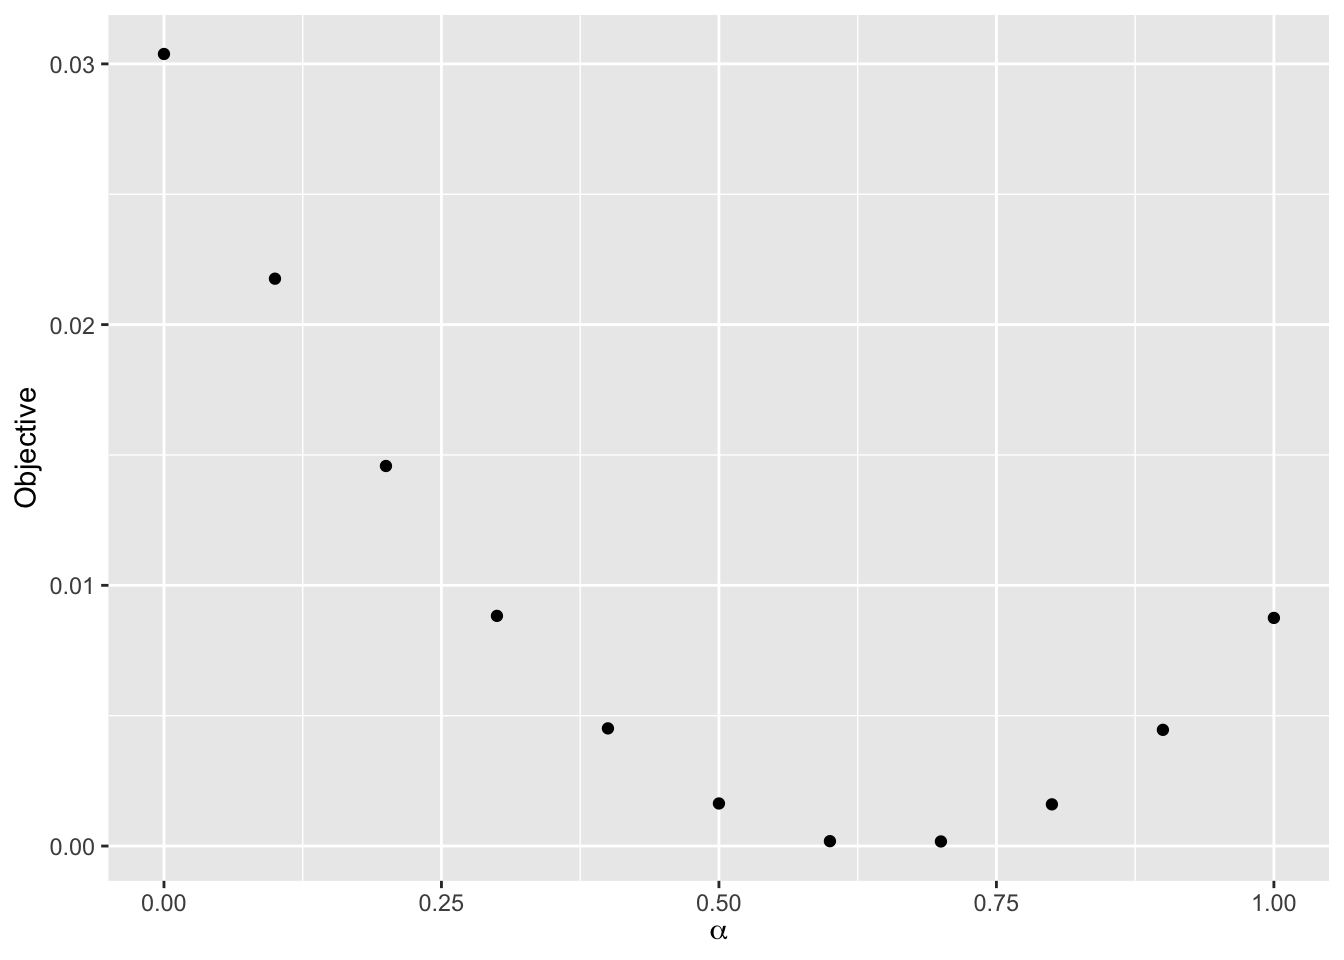
\includegraphics{6-assignment-solution_files/figure-latex/unnamed-chunk-23-1} \end{center}

\end{document}
